\chapter{Prediction-Based Scheduler}\label{chap:prediction_based_scheduler}

\section{Overview}
\label{pbs:overview}
In this chapter, we present the foundation of the prediction-based scheduler. The problem defined here is the primary motivation for the current work and the anchor for the dissertation outline in Chapter \ref{chap:outline}. The work presented in Chapter \ref{chap:prediction_based_scheduler} is taken from \cite{ravan_ensuring_2020}.

\section{Introduction}
\label{pbs:introduction}
Consistency among multiple interleaved transactions in a web service context has always been an issue for researchers and database administrators. Isolation and atomicity are two of the four \ac{ACID}\footnote{The four traditional database properties are Atomicity, Consistency, Isolation, and Durability} properties that are often relaxed in order to prevent a performance bottleneck. However, when these properties are relaxed, the database can reach an inconsistent state when concurrent transactions interleave incorrectly. This causes data to become corrupted, expensive compensation transactions to be executed, and cascading rollbacks on multiple nodes to be completed before processing can continue. By looking at a practical use case we can more clearly see the issue and the need for a solution that ensures consistency. In Figures \ref{fig:e_com_ticket} \& \ref{fig:bp_env}, we see five web services executing on three different database instances. The first four web services  create a common business process created by the Business Process Execution Language (\ac{BPEL}) \cite{BPEL}. The web services are: $WS_{1}$ (decrement inventory by product ID), $WS_{2}$ (process payment), $WS_{3}$ (add order by user ID), and $WS_{4}$ (delete user payment info). The goal of the process is to allow a customer to purchase a product from an e-Commerce site. $WS_{5}$ (delete user payment info) and $WS_{3}$ execute within the same database instance. With the relaxed properties in the web service context, concurrent executions of $WS_{5}$ and $WS_{3}$ could cause an inconsistent state on $Node_{3}$. This would then cause a cascading rollback to execute and revert the committed operations of $WS_{1}$ and $WS_{2}$. Existing research shows that many solutions have been presented in the past to address this issue (e.g., \cite{Fekete_SnapshotIso}, \cite{Alrifai_Distributed_Managment}, \cite{Fekete_RAMP}, \cite{Fekete_IsolationSupport}, \cite{Jacobi_Locking}, and \cite{Fekete_Promises}). The most influential research that inspired the prediction-based solution was the Promises Model.

The Promises model presented by Alan Fekete et al. (e.g., \cite{Fekete_IsolationSupport} and \cite{Fekete_Promises}) is an elegant solution that "promises" a particular transaction that the requested resource will be available while allowing concurrent transactions to still execute on that resource. The Promises solution is robust in that it allows the "strengthening" or "weakening" of promises after they have already been made. This allows existing promises on resources to be modified without breaking the existing promise entirely. However, the solution introduces backwards compatibility issues along with a potential bottleneck at the occurrence of registering a promise for a particular transaction. 

Our prediction-based solution allows transactions to build a reputation linked to a category (categories are defined in Definition \ref{transaction_categories} \& \ref{cat_dominance}). The priorities associated with the category impact the transaction's scheduling in order to prevent cascading rollbacks. There are lock behaviors associated with the categories that enable preemptive scheduling in order to increase efficiency. The contributions in the prediction-based solution address the two issues of efficiency and consistency where existing research solutions fall short. Section \ref{pbs:problem_def} outlines the problem along with a use-case scenario. Section \ref{pbs:related_work} discusses the existing research that has already taken place in regards to the problem. Section \ref{pbs:system_model} outlines the system model for the solution. Section \ref{pbs:algorithms} discusses the algorithms needed for the solution and their psuedocode. Section \ref{pbs:analysis} provides the formal proofs for the given solution. Section \ref{pbs:experimentation} illustrates the simulation results gathered from the prototype.
\section{Problem Definition}
\label{pbs:problem_def}
Transactions in traditional database systems satisfy the four ACID  properties: Atomicity, Consistency, Isolation, and Durability. ACID transactions guarantee leaving the database in a consistent state. However, in a web service environment ACID properties and transactional concurrency cannot be fulfilled, due to performance issues. Common occurrences in web service environments involve the collaboration of multiple web services to fulfill a particular task without coupling all the needed operations in one service. Languages, such as BPEL (Business Process Execution Language) \cite{BPEL}, allow a large majority of these business processes to execute web services that must access the underlying database management systems (DBMS). These transactions may be required to relax the isolation property of the database in order to accommodate concurrent transactions.

In the event that a transaction fails (abort), and there are transactions depending on the successful execution of the failed transaction, a cascading rollback must occur, due to the inconsistency of the database. This occurs often in the web service environment due to the relaxed atomicity and isolation properties. The relaxation of the atomicity property allows operations within a transaction to commit any changes performed by the operation permanently before the entire transaction has been completed. The relaxation of the isolation property allows the interleaved execution of operations on a particular resource from concurrent transactions. This improves performance tremendously; however, in the event an operation fails, causing an abort to be issued, every transaction depending upon the failed operation must be aborted as well in order to restore consistency. These compensation transactions have become a standard practice in web service environments but sacrifice the consistency of the system. The next section will discuss a use-case scenario where this problem exists.

\subsection{Use-Case Scenario}
\label{subsec:use_case}
Assume that an e-commerce web site allows users to purchase products through an online interface. When a customer places an order a ticket is generated (see Figure \ref{fig:e_com_ticket}) containing information about the user and purchase. The ticket from the site is then handed off to a business process (starting at $WS_{1}$ in Figure \ref{fig:bp_env}) containing multiple web services, on multiple databases in a distributed context. Figure \ref{fig:bp_env} displays the architecture of the back-end business process in sequence.

\begin{figure}[h]
\captionsetup{justification=centering}
\centering % used for centering Figure

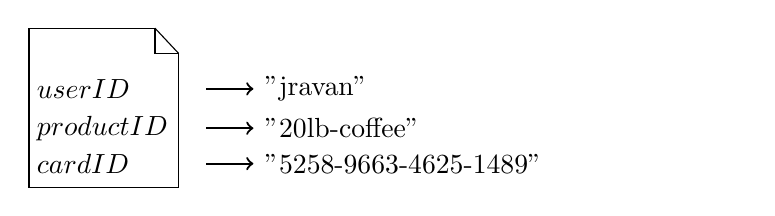
\begin{tikzpicture}
  \draw (0,0) -- (0,2.02) -- (1.6,2.02) -- (1.6,1.7) -- (1.9,1.7) -- (1.9,0) -- cycle;
  \draw (1.6,2.02) -- (1.9,1.7);
  \node[text width=1.5cm] at (.85,1.25) {$userID$};
  \node[text width=1.5cm] at (.85,.75) {$productID$};
  \node[text width=1.5cm] at (.85,.3) {$cardID$};
  \draw[thick,->] (2.25,1.25) -- (2.85,1.25);
  \draw[thick,->] (2.25,.75) -- (2.85,.75);
  \draw[thick,->] (2.25,.3) -- (2.85,.3);
  \node[text width=6cm] at (6,1.25) {"jravan"};
  \node[text width=6cm] at (6,.75) {"20lb-coffee"};
  \node[text width=6cm] at (6,.3) {"5258-9663-4625-1489"};
\end{tikzpicture}

\caption{e-Commerce Web Site Ticket Example} % title of the Figure
\label{fig:e_com_ticket} %% label to refer figure in text

\end{figure}

\begin{figure}[h]
\captionsetup{justification=centering}
\centering % used for centering Figure

\begin{tikzpicture}
    \node [webservice, anchor=north] (ws4) {$WS_{4}$};
    \node [webservice, above=2cm of ws4.north, anchor=north] (ws3) {$WS_{3}$};
    \node [webservice, above=2cm of ws3.north, anchor=north] (ws2) {$WS_{2}$};
    \node [webservice, above=2cm of ws2.north, anchor=north] (ws1) {$WS_{1}$};
    \node [draw, cylinder, shape border rotate=90, aspect=0.75, %
      minimum height=30, minimum width=30, anchor=north, left=.5cm of ws3] (data3) {DB};
    \node [draw, cylinder, shape border rotate=90, aspect=0.75, %
      minimum height=30, minimum width=30, above=2cm of data3.north, anchor=north] (data2) {DB};
    \node [draw, cylinder, shape border rotate=90, aspect=0.75, %
      minimum height=30, minimum width=30, above=2cm of data2.north, anchor=north] (data1) {DB};
    \node [webservice, left=4cm of ws3.north, anchor=north] (ws5) {$WS_{5}$};
    \path [line] (ws1) -- (data1);
    \path [line] (ws2) -- (data2);
    \path [line] (ws3) -- (data3);
    \path [line] (ws1) -- (ws2);
    \path [line] (ws2) -- (ws3);
    \path [line] (ws3) -- (ws4);
    \path [line] (ws5) -- (data3);
    \draw[dotted,blue] (-5.25,.35) rectangle (3,-1.55);
    \draw[dotted,red] (-5.25,2.35) rectangle (3,.45);
    \draw[dotted,black] (-5.25,4.35) rectangle (3,2.45);
    \draw[dotted,purple] (-5.25,6.35) rectangle (3,4.45);
    \node[text width=1cm] at (2,6) {$Node_{1}$};
    \node[text width=1cm] at (2,4) {$Node_{2}$};
    \node[text width=1cm] at (2,2) {$Node_{3}$};
    \node[text width=1cm] at (2,0) {$Node_{4}$};
    \node[text width=9cm] at (-.5,-2) {$WS_{1} = Decrement Inventory By Product ID$};
    \node[text width=7cm] at (-.5,-2.5) {$WS_{2} = Process Payment$};
    \node[text width=7cm] at (-.5,-3) {$WS_{3} = Get Order By User ID$};
    \node[text width=7cm] at (-.5,-3.5) {$WS_{4} = Generate Receipt$};
    \node[text width=7cm] at (-.5,-4) {$WS_{5} = Delete Order By User ID$};
\end{tikzpicture}

\caption{Business Process for e-Commerce Web Site} % title of the Figure
\label{fig:bp_env} % label to refer figure in text

\end{figure}

Each dotted rectangle within Figure \ref{fig:bp_env} represents a distributed node containing a public web service executing transactions on an underlying database. In order for a successful purchase to take place within the e-commerce environment, the business process containing the web service sequence $WS_{1}, WS_{2}, WS_{3},$ and $WS_{4}$ must execute successfully. $WS_{1}$ ($DecrementInventoryByProductID$) uses the $productID$ provided from the current ticket in order to query the database regarding the requested product. $WS_{2}$ ($ProcessPayment$) uses the payment information provided in the ticket to charge the user. $WS_{3}$ ($GetOrderByUserID$) is a service that takes the given $userID$ and $product ID$, and returns a record of purchase for the user. $WS_{4}$ ($GenerateReceipt$) simply generates a receipt from the ticket information and is returned to the user's interface. Once $WS_{4}$ has completed processing, and only when it is finished, a purchase is considered successful.

The issue is that multiple web services may be executed on a single database instance. Without concurrency control, interleaved executions, such as the case with $WS_{3},$ and $WS_{5}$, may cause inconsistencies. 

% \subsection{Use Case Transactions for $Node_{3}$}
% \label{sec:use_case_for_node_3}
% In Figure \ref{fig:webform}, we see the contents of the two transactions executing on $Node_{3}$. $T_{DeleteOrderByUserID}$ is a transaction generated by $W_{5}$. The responsibility of this web service is to determine if the user exists, and if they do exist, to delete the user's order information from the database by the provided \textit{userID}. The transaction generated by $WS_{3}$ ($T_{GetOrderByUserID}$, mentioned above from Figure \ref{fig:bp_env}) is responsible for getting an order from a user account. This transaction executes under the pretext that the \textit{userID} given exists in the database or the web service would not have been able to be executed. If $T_{GetOrderByUserID}$ fails within the business process outlined in Figure \ref{fig:bp_env}, then an abort must be issued, and all the previous operations committed from $WS_{1}$ and $WS_{2}$ must be rolled back. This includes operations that were executed from subsequent transactions that depended on the results of $WS_{1}$ and $WS_{2}$.

Assume $WS_{3}$ and $WS_{5}$ are $T_{GetOrderByUserID}$ and $T_{DeleteOrderByUserID}$. The deletion transaction contains four operations: $R_{2}(b)$, $W_{2}(b)$, $R_{2}(a)$, and $W_{2}(a)$. The transaction will first READ from the database to ensure the user exists and then WRITE out the order information if the order does exist\footnote{In this instance the WRITE operation executed would write a $NULL$ or empty record to the database in order to "delete" the record.}. The other transaction, $T_{GetOrderByUserID}$, contains a single $R_{1}(a)$ and $R_{1}(b)$. Each transaction contains a $C_{i}$ operation that represents the COMMIT operation that the database executes after all operations have completed. Figure \ref{fig:webform} shows the two transactions along with the operations contained within.

\begin{figure}[h]
\captionsetup{justification=centering}
\centering % used for centering Figure

\begin{picture}(50,40)
    \put(-80.5,25){$W_{3} = T_{GetOrderByUserID}$ = $R_{1}(a)R_{1}(b)C_{1}$}
    \put(-97,10){$W_{5} = T_{DeleteOrderByUserID}$ = $R_{2}(b)W_{2}(b)R_{2}(a)W_{2}(a)C_{2}$}
\end{picture}

\caption{e-Commerce Web Service Transaction Sequences} % title of the Figure
\label{fig:webform} % label to refer figure in text

\end{figure}

% \subsection{Use Case Transaction Metrics}
For the transactions listed above, we know the commit rate, number of transactions executed, and the average execution time. Commit rate is the percentage of successful commits over the total amount of attempted executions of that particular transaction (Definition \ref{cmt_rate}). Number of transactions represents the total number of executions attempted (commits and aborts combined) for that particular transaction. Efficiency rate represents the average efficiency of the particular transaction to reach a completion state; whether it is a failure or success (Definition \ref{eff_rate}). A transaction with a very long execution time will have an efficiency rate that is much lower than a transaction that executes and completes very quickly. The attribute data listed previously is consolidated into Table \ref{tbl:trans_metrics} below. 
\\
\begin{table}[h]
\captionsetup{justification=centering}
\centering
\begin{tabular}{|c|c|c|c|c|}
\hline
\multicolumn{4}{|c|}{\cellcolor[HTML]{EFEFEF}\textbf{Transaction Metrics}}                                                   \\ \hline
\textbf{Transactions} & \textbf{Commit Rate} & \textbf{\# of Trans.} & {\color[HTML]{000000} \textbf{Eff. Rate}} \\ \hline
$T_{DeleteOrderByUserID}$         & 98\%                  & 200                         & 98\%                                          \\ \hline
$T_{GetOrderByUserID}$          & 97\%                     & 520                           & 99\%                                              \\ \hline
\end{tabular}

\caption{Transaction Metrics} % title of the Figure
\label{tbl:trans_metrics} % label to refer figure in text

\end{table}

In a web service context, without the prediction-based solution, the isolation property will be relaxed and a serializable execution will be created. This serializable execution will be based on the conflicting operations of the two transactions. Figure \ref{fig:combined_history} displays an example of a generated serializable execution from $T_{GetOrderByUserID}$ and $T_{DeleteOrderByUserID}$.

\begin{figure}[h]
\captionsetup{justification=centering}
\centering % used for centering Figure

\begin{picture}(50,25)
    \put(-90,5){$T_{Schedule}$ = $R_{1}(a)R_{2}(b)R_{1}(b)W_{2}(b)R_{2}(a)W_{2}(a)$}
\end{picture}

\caption{Generated Schedule} % title of the Figure
\label{fig:combined_history} % label to refer figure in text

\end{figure}

The schedule listed in Figure \ref{fig:combined_history} is a well-formed serializable schedule. Between each operation within the schedule, a commit operation $C_{i}$ is executed. This shows how the Atomcity property of a database is relaxed during the execution of a schedule. Therefore, if $R_{2}(a)$ fails, a cascading rollback will be issued causing the operations of $T_{GetOrderByUserID}$ to be rolled back regardless of their successful execution. The operations of $T_{GetOrderByUserID}$ must be rolled back since they are a part of $T_{Schedule}$ and a COMMIT operation has been executed already. If $T_{GetOrderByUserID}$ was executed as a part of the business process outlined in the use case, then the operations of the previous web services ($WS_{1}$ and $WS_{2}$) must be rolled back.

Conversely, if the data in Table \ref{tbl:trans_metrics} were taken into consideration before generating the serializable execution, $T_{GetOrderByUserID}$ could be given a more restrictive concurrency control mechanism, such as locking. Table \ref{tbl:trans_metrics} contains data that proves instances of $T_{GetOrderByUserID}$ have a high rate of commit with a high percentage of efficiency throughout the system. Table \ref{tbl:trans_metrics} also displays that instances of $T_{DeleteOrderByUserID}$ could use locking techniques due to its history. Therefore, $T_{GetOrderByUserID}$ and $T_{DeleteOrderByUserID}$ could execute within the same schedule using traditional locking techniques, commit changes quickly and successfully, and prevent a cascading rollback from reverting the effects of $WS_{1}$ and $WS_{2}$ by using the reputation provided by the separate transactions. In the proposed solution, we aim to provide concurrency control that is based on the metadata of the transactions. Our hypothesis is that if transactions could be treated differently based on their history, stronger concurrency control techniques could be leveraged, such as locking, which ensures the consistency property for web service transactions. Section \ref{pbs:analysis} walks through this exact use-case scenario with two-phase locking and the proposed prediction-based solution. The next section will discuss the existing research that has taken place to remediate this problem without the current knowledge of transaction metrics.
\section{Related Work}
\label{pbs:related_work}

Ensuring successful concurrency control in web service transactions has been studied in depth for some time (e.g., \cite{Fekete_Promises}, \cite{Fekete_IsolationSupport}, \cite{Alrifai_Distributed_Managment}, \cite{dai_qos-driven_2009}, \cite{zhengdong_gao_combining_2005}, \cite{ferreira_transactional_2012}, \cite{kang-woo_lee_consistency_2000}, and \cite{olmsted_long_2015}). The Promises model presented by Alan Fekete et al. (e.g., \cite{Fekete_Promises} and \cite{Fekete_IsolationSupport}) is an elegant solution that "promises" a particular transaction that the requested resource will be available while allowing concurrent transactions to still execute on that resource. Alomari et al. present a solution involving an External Lock Manager (\gls{elm}) that resides outside of the \gls{dbms} \cite{Fekete_SnapshotIso}. This allows a layer of separation between the application and the \gls{dbms} in order to schedule transactions using special business logic according to the environment. In the solution presented by Alrifai et al. \cite{Alrifai_Distributed_Managment}, an edge chasing solution using dependency graphs is incorporated in order to detect dependencies between globally scheduled transactions. The solution was tested parallel to the well known 2-Phase Locking Protocol (\gls{2pl}) and provided promising results regarding efficiency. However, the Alrifai et al. solution becomes less efficient when the number of dependency cycles are detected. The model of the different lock types comes from Christian Jacobi et al. \cite{Jacobi_Locking} with research in concurrent locking with parallel database systems. The researchers extended the use of the native lock types in the existing database structure in order to speed up thread processing on multi-processor machines. Prediction-based concurrency control has been proposed by Eunhee Lee et al. \cite{Eunhee_PredictionBasedCC} with the entity-radius solution. This solution uses the concept of multiple entity radii that attempts to predict the next user based on their location. The prediction is generated from the location within a radius of the replicated site and their navigation speed. The solution provided is elegant with excellent experimental results but no formal proof or analysis of the algorithm is provided. Other solutions to prevent business process cancellation or rollback when participants of the process do not behave correctly involve global views of the process \cite{Fekete_RAMP}, \cite{Riegen_RuleBased}. Support for these types of solutions are based on the well-known Oasis specifications of WS-Coordination, WS-AtomicTransaction, and WS-BusinessActivity \cite{WSCO}, \cite{WSAT}, \cite{WSBA}. These solutions are well-designed; however, they require the presence of a global coordinator throughout the entire business process. In the next section, we will discuss the prediction-based solution's system model generated from the current available work in the research community.

%%%%%% BEGINNING OF SYSTEM MODEL SECTION %%%%%%%
\section{System Model}
\label{pbs:system_model}
This section outlines the system model on which the solution is built. Definitions for new concepts are introduced first, considering they will be used to describe the different components that consist of the system model. Later subsections explain in detail the different components and processes required for the prediction-based solution. We assume that all the transactions are well-formed and the scheduler is legal.

\subsection{Definitions}
\label{pbs:definitions}

\defCommitRate{cmt_rate}
\defEfficiencyRate{eff_rate}

\begin{definition}
\label{cat_bounds}
 (Categorization Thresholds) - categorization thresholds are upper and lower limits of both commit rate and efficiency rate that are used when categorizing transactions\footnote{The categorization bounds are static values that do not change throughout the system execution. Both the efficiency rate and the commit rate bounds are currently at 50\% creating full coverage of all transactions.}.
\end{definition}

% \begin{definition}
% \label{cat_threshold}
%  (Categorization Thresholds) - categorization thresholds are calculated within the categorization bounds (see Definition \ref{cat_bounds}) by using the Transaction Concentration Ratio (see Section \ref{sec:TCR}). The threshold values are dynamic and change depending on the execution environment but will not exceed the categorization bounds placed on that particular category. Categorization thresholds enforce the most accurate thresholds for the execution environment while allowing flexibility.
% \end{definition}

\begin{definition}
\label{transaction_categories}
(Transaction Categories) - Let $T$ = \{$T_{1}$, ... , $T_{n}$\} be a set of transactions and $C$ = \{$HCHE$, $HCLE$, $LCHE$, $LCLE$\} a set of category names. The mapping $\tau$ associates a category name with each transaction as follows:

\[ 
\tau : \textrm{$T_{i}$}\rightarrow
\left \{
  \begin{tabular}{cc}
  HCHE & if $C_{r}(T_{i}) > 0.5$ and $E_{r}(T_{i}) > 1$ \\
  HCLE & if $C_{r}(T_{i}) > 0.5$ and $E_{r}(T_{i}) \le 0.5$ \\
  LCHE & if $C_{r}(T_{i}) \le 0.5$ and $E_{r}(T_{i}) > 1$ \\
  LCLE & if $C_{r}(T_{i}) \le 0.5$ and $E_{r}(T_{i}) \le 0.5$
  \end{tabular}
\right \}
\]

{\normalfont In order to ensure correct lock techniques are selected, transactions cannot be simply characterized as good or bad based on their metrics. For example, a transaction $T_{1}$ may have a 100\% commit rate, but it may have a long execution time. A transaction with these characteristics should not be penalized when, in fact, it is a well behaving transaction. On the other hand, a transaction $T_{2}$ that has a 100\% commit rate and has an extremely short execution time should not be treated with the same priority as $T_{1}$. This is where certain of levels must be established to ensure the most appropriate selection is made.

In order to establish levels, a system of categories was put in place base on the metrics mentioned previously. The first categorization is based solely on the efficiency of the transaction. In this categorization, there are two attributes: \textit{high efficiency (HE)} and \textit{low efficiency (LE)}. A transaction that has been labeled as \textit{HE} is considered to execute with an efficiency in the upper 50\% of all transactions executed within the system\footnote{See Section \ref{pbs:cat_graph} and Section \ref{pbs:definitions} for more clarification}. The second attribute, \textit{LE}, is any transaction where its efficiency rate is in the lower 50\% of all transactions executed.

The second categorization that the levels are built on is based solely on the outcome of the transaction. These attributes are \textit{high commit (HC)} and \textit{low commit (LC)}, which are much more simple to define. A transaction with a \textit{HC} attribute has committed successfully over 50\% of executions (upper 50\% of all transactions). A transaction with an \textit{LC} attribute has failed over 50\% of its executions (lower 50\% of all transactions). This categorization correlates directly with the commit rate defined (see Definition \ref{cmt_rate}).

With these two categorizations and two attributes, a four-level system was devised in order to select appropriate lock types. The four categories devised are \textit{high commit-high efficiency (HCHE)}, \textit{high commit-low efficiency (HCLE)}, \textit{low commit-high efficiency (LCHE)}, and \textit{low commit-low efficiency (LCLE)}. Depending on the level in which the transaction has been placed, different lock types will be granted in order to perform concurrency control.}

\end{definition}

\begin{definition}
\label{cat_dominance}
(Transaction Category Dominance) - The Transaction Category Dominance is a pair, denoted as $C_{D} = (C,L)$, where $C$ is the set of transaction categories, and $L$ is a partial order of the categories such that:
 
\[\textrm{$HCHE > HCLE > LCLE$}\]
\[\textrm{$HCHE > LCHE > LCLE$} \]

\begin{figure}[h]
\captionsetup{justification=centering}
\centering % used for centering Figure

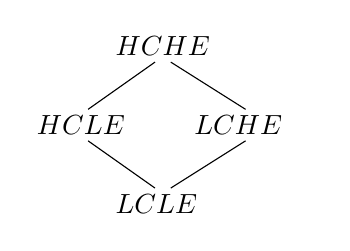
\begin{tikzpicture}
    % [list/.style={rectangle split, rectangle split parts=3,
    % draw, rectangle split horizontal}, >=stealth, start chain]
  \node[text width=1.5cm] at (3.8,5) {$HCHE$};
  \node[text width=1.5cm] at (2.8,4) {$HCLE$};
  \node[text width=1.5cm] at (4.8,4) {$LCHE$};
  \node[text width=1.5cm] at (3.8,3) {$LCLE$};
  \draw (3.55,4.8) -- (2.7,4.2);
  \draw (3.75,4.8) -- (4.7,4.2);
  \draw (3.55,3.2) -- (2.7,3.8);
  \draw (3.75,3.2) -- (4.7,3.8);
  
\end{tikzpicture}

% \caption{Web Service Environment with Scheduler} % title of the Figure
\label{fig:category_lattice} % label to refer figure in text

\end{figure}

{\normalfont Note that the categories $HCLE$ and $LCHE$ are not comparable. That is, we cannot establish a dominance relation between transactions in $HCLE$ and $LCHE$ categories.

However, in our model, we focus on reducing the need of compensation for aborted transactions. Therefore, we prioritize the commit property over the efficiency property. We introduce the dominance relation below in Table \ref{tbl:priority}.}

\[\textrm{$HCLE > LCHE$} \]
 
\begin{table}[h]
\captionsetup{justification=centering}
\centering
\begin{tabular}{l|c|}
\cline{2-2}
                                          & \multicolumn{1}{l|}{\textbf{Priority}} \\ \hline
\multicolumn{1}{|l|}{\textbf{HCHE}}  & I                                      \\ \hline
\multicolumn{1}{|l|}{\textbf{HCLE}}  & II                                     \\ \hline
\multicolumn{1}{|l|}{\textbf{LCHE}} & III                                     \\ \hline
\multicolumn{1}{|l|}{\textbf{LCLE}} & IV                                      \\ \hline
\end{tabular}

\caption{Category Priorities} % title of the Figure
\label{tbl:priority} % label to refer figure in text

\end{table} 

\end{definition}

% \begin{definition}
% \label{min_commit}
% (HCHE) - HCHE, acronym for High Commit High Efficiency, is a transaction categorization with categorization bounds (see Definition \ref{cat_bounds}) that involve a commit rate of 50\% and higher and a efficiency rate in the upper 50\% and higher as well (see Definitions \ref{cmt_rate} and \ref{eff_rate}). Table \ref{tbl:default_tmetrics} outlines all transaction categories.
% \end{definition}

% \begin{definition}
% \label{min_abrt}
% (LCHE) - LCHE, acronym for Low Commit High Efficiency, is a transaction categorization with categorization bounds (see Definition \ref{cat_bounds}) that involve a commit rate of 50\% and lower and a efficiency rate in the upper 50\% and higher (see Definitions \ref{cmt_rate} and \ref{eff_rate}). Table \ref{tbl:default_tmetrics} outlines all transaction categories.
% \end{definition}

% \begin{definition}
% \label{ext_commit}
% (HCLE) - HCLE, acronym for High Commit Low Efficiency, is a transaction categorization with categorization bounds (see Definition \ref{cat_bounds}) that involve a commit rate of 50\% and higher and a efficiency rate in the bottom 50\% and lower (see Definitions \ref{cmt_rate} and \ref{eff_rate}). Table \ref{tbl:default_tmetrics} outlines all transaction categories.
% \end{definition}

% \begin{definition}
% \label{ext_abrt}
% (LCLE) - LCLE, acronym for Low Commit Low Efficiency, is a transaction categorization with categorization bounds (see Definition \ref{cat_bounds}) that involve a commit rate of 50\% and lower and a efficiency rate in the bottom 50\% and lower as well (see Definitions \ref{cmt_rate} and \ref{eff_rate}). Table \ref{tbl:default_tmetrics} outlines all transaction categories.
% \end{definition}

%\begin{definition}
%\label{no_trend}
%(NO\_TREND) - NO\_TREND is a transaction categorization with categorization bounds (see Definition \ref{cat_bounds}) that include all %the outlining space that the previous four categories do not include. If the efficiency rate is less than or equal to 25\% then the %commit rate must be between 25\% and 75\% (see Definitions \ref{cmt_rate} and \ref{eff_rate}). If the efficiency rate is between 25\% %and 75\% then the commit rate includes all values ranging from 0\% to 100\%. Finally, if the efficiency rate is greater than or equal %to 75\% then the commit rate must be between 25\% and 75\%. Table \ref{tbl:default_tmetrics} outlines all transaction categories.
%\end{definition}

%\[
%\left \{
%  \begin{tabular}{ll}
%  
%  $E_{r}\le25\%$, & $25\%<C_{r}<75\%$ \\
%  $25\%<E_{r}<75\%$, & $0\%\le C_{r}\le100\%$ \\
%  $E_{r}\ge75\%$, & $25\%<C_{r}<75\%$
%  
%  \end{tabular}
%\right \}
%\]

\begin{definition}
\label{conflict_ops}
 (Conflicting Operations) - two operations are conflicting:

 \begin{enumerate}
   \item they are contained within two different transactions,
   \item both operations are operating on the same data item, and
   \item at least one of the operations is a WRITE
 \end{enumerate}

 \begin{example}
 \label{ex_conflict_ops}
  Let $o_{1}$ be a READ operation on data item $User ID$ in transaction $T_{1}$ and let $o_{2}$ be a WRITE operation on $User ID$ in $T_{2}$. These two operations are conflicting.
 \end{example}
\end{definition}

% \begin{definition}
% \label{conflict_trans}
%  (Conflicting Transactions) - two transactions are considered conflicting if they contain all of the following attributes:
 
%  \begin{enumerate}
%  \item both transactions contain conflicting operations (see Definition \ref{conflict_ops})
%  \item both transactions are contained within the same serializable schedule
%  \item and at least one of the transactions is categorized to abort
%  \end{enumerate}
 
%  \begin{example}
%  \label{ex_conflict_trans}
%   Using the transactions mentioned in Example \ref{ex_conflict_ops} let's say the serializable schedule $S_{1}$ contains   an interleaved execution of $T_{1}$ and $T_{2}$. These transactions are now considered conflicting.
%  \end{example}
% \end{definition}

% \begin{definition}
% \label{conflict_cat}
%   (Conflicting Categories) - conflicting categories are very much related to conflicting transactions (see Definition \ref{conflict_trans}) however this definition is concerned with the categories the transactions have been placed in rather than the transactions themselves. Two categories are said to be conflicting if they contain all of the following attributes:
  
%   \begin{enumerate}
%   \item both are contained within the same serializable schedule
%   \item and at least one of the categories is predicted to abort
%   \end{enumerate}
  
% Transactions of conflicting categories are not allowed within the same schedule within this solution.  
  
%   \begin{example}
%   For example, let's say we have transaction $T_{1}$ that has been placed in the category HCHE and transaction $T_{2}$ that has been placed in the category LCLE. These two categories are considered conflicting even if $T_{1}$ and $T_{2}$ are not considered to be conflicting transactions themselves.
%   \end{example}
  
% \end{definition}

% \begin{definition}
% \label{serial_sched}
%  (Serializable Schedule) - a serializable schedule is a non-serial schedule that can be converted to a serial schedule by interchanging non-conflicting operations (see Definition \ref{conflict_ops})

% \end{definition}

% \begin{definition}
% \label{casc_rollback}
%  (Cascading Rollback) - a cascading rollback occurs when two conflicting transactions (see Definition                     \ref{conflict_trans}) are interleaved within the same serializable schedule. The abort is cascading in the sense that an  abort must be issued for each transaction within the schedule that was dependant upon the transaction that issued the abort. This is needed to ensure a consistent state within the database.
 
%  \begin{example}
%  \label{ex_casc_rollback}
%   Using the serializable schedule generated in Example \ref{ex_conflict_trans}, if transaction $T_{2}$ issues an abort then  transaction $T_{1}$ must also be aborted since $T_{1}$ is dependant upon $T_{2}$.
%  \end{example}
 
% \end{definition}

\begin{definition}
\label{compatibility}
(Compatibility) - a data item is locked in a non-compatible mode if:

\begin{enumerate}
  \item the data item is locked by write-lock, or
  \item the data item requesting the lock is categorized with a lower priority
\end{enumerate}
\end{definition}

\begin{definition}
\label{legal_scheduler}
 (Legal Scheduler) - a prediction-based scheduler is legal if:
 
 \begin{enumerate}
    \item \textbf{Grant:} (denoted as the addition symbol, +) a transaction is permitted to lock a data item if the data item is not already locked in a non-compatible mode (see Definition \ref{compatibility}) by an other transaction\footnote{In the event that a lock is requested of a resource that has not issued any locks, then the lock will be automatically granted. There is no conflict, and therefore, the compatibility matrices do not apply.}.
    \item \textbf{Decline:} (denoted as the subtraction symbol, -) a transaction $T_{i}$ is denied to lock a data item if the data item is already locked in a non-compatible mode (see Definition \ref{compatibility}) by another transaction $T_{j}$ where $\tau(T_{i}) \le \tau(T_{j})$
    \item \textbf{Elevate:} (denoted as lowercase delta, $\delta$) a transaction $T_{i}$ is permitted to lock a data item if all the non-compatible locks (see Definition \ref{compatibility}) on the data item are being held by transactions $T_{1}, ... , T_{k}$ such that $\tau(T_{j}) < \tau(T_{i})$ for all $j = 1, ..., k$ in this case $T_{1}, ... , T_{k}$ must first release the locks on the data item before $T_{i}$ is permitted to lock the data item.
 \end{enumerate}

% \begin{definition}
% \label{grant_action}
%  (Grant Action) - the grant action is one of the three possible actions that can take place within the two lock compatibility matrices (Table \ref{tbl:read_lock_compatibility} \& Table \ref{tbl:write_lock_compatibility}). This action is represented by the plus sign (+) which signifies that there is not a conflict between the granted and requesting transactions and the lock can be granted to the transaction that is requesting access to the resource.
 
 \begin{example}
 \label{ex_grant_action}
  A read-lock for a data item $R$ has been granted to transaction $T_{1}$ within the $HCHE$ transactional category. Transaction $T_{2}$ within the $HCLE$ is also requesting a read-lock on data item $R$. This does not cause a conflict and therefore the grant action will be taken and the requested lock will be issued to $T_{2}$.
 \end{example}
 
% \end{definition}

% \begin{definition}
% \label{decline_action}
%  (Decline Action) - the decline action is one of the three possible actions that can take place within the two lock compatibility matrices (Table \ref{tbl:read_lock_compatibility} \& Table \ref{tbl:write_lock_compatibility}). This action is represented by the minus sign (-) which signifies that there is a conflict between the granted and requesting transactions and the lock can not be granted to the transaction that is requesting access to the resource.
 
 \begin{example}
 \label{ex_decline_action}
  A write-lock for a data item $R$ has been granted to transaction $T_{1}$ within the $HCHE$ transactional category. Transaction $T_{2}$ within the $HCLE$ is requesting a write-lock to data item $R$. This causes a conflict and therefore the decline action will be taken and the requested lock will not be issued to $T_{2}$.
 \end{example}
 
% \end{definition}

% \begin{definition}
% \label{elevate_action}
%  (Elevate Action) - the elevate action is one of the three possible actions that can take place within the two lock compatibility matrices (Table \ref{tbl:read_lock_compatibility} \& Table \ref{tbl:write_lock_compatibility}). This action is represented by the delta symbol ($\delta$) which signifies that the transaction requesting access to the resource is in a category that contains a higher prioritization (see Table \ref{tbl:priority}) than the transactions that currently hold locks to the resource. In this situation all locks held by transactions of lower priority will be preemptively dropped so the transaction with the higher priority can obtain the needed lock.
 
 \begin{example}
 \label{ex_elevate_action}
  A read-lock for a data item $R$ has been granted to transaction $T_{1}$ within the $LCLE$ transactional category. Transaction $T_{2}$ within the $HCHE$ is requesting a write-lock to data item $R$. However, this causes a conflict; since $T_{2}$ contains a higher priority than $T_{1}$; the elevate action will be taken and the requested lock will be issued to $T_{2}$.
 \end{example}
 
\end{definition}
\subsection{Environment}
\label{pbs:environment}
In a web services environment, multiple web services can submit transactions to a database to be executed. As mentioned before, if only one transaction can be executed at any given time, then other concurrent transactions from other web services must wait. This causes a significant performance degradation; therefore, concurrent transactions from multiple web services must be handled. This is where the Database Management System's (\ac{DBMS}) scheduler plays an important role in ensuring concurrent transactions preserve consistency within the database. The scheduler receives transactions that are submitted from web services and generates a serializable schedule based on the conflicting operations contained within the transactions. 

After receiving the concurrent transactions (e.g., $T_{1}$, $T_{2}$, ... , $T_{N}$) the scheduler is responsible for analyzing the conflicting operations within the transactions and generating a serializable schedule that will then be executed on the database itself (e.g., $T_{Sched}$). This serializable execution is guaranteed to leave the database in a consistent state after a successful execution due to the analysis performed by the scheduler and the ordering of the operations within the transaction. Figure \ref{fig:Tsched} displays the generation of $T_{Sched}$ from multiple web service transactions. Figure \ref{fig:ws_env} displays a diagram of the database scheduler in a web service context.

\begin{figure}[h]
\captionsetup{justification=centering}
\centering % used for centering Figure

\begin{picture}(55,100)
    \put(-93,80){$T_{1}$ = \{ $W_{1}(r_{1})R_{1}(r_{1})W_{1}(r_{2})R_{1}(r_{2})$ ... $W_{1}(r_{n})R_{1}(r_{n})C_{1}$ \}}
    \put(-93,65){$T_{2}$ = \{ $W_{2}(r_{1})R_{2}(r_{1})W_{2}(r_{2})R_{2}(r_{2})$ ... $W_{2}(r_{n})R_{2}(r_{n})C_{2}$ \}}
    \put(-58,50){.}
    \put(-58,45){.}
    \put(-58,40){.}
    \put(-100,23){$T_{N}$ = \{ $W_{n}(r_{1})R_{n}(r_{1})W_{n}(r_{2})R_{n}(r_{2})$ ... $W_{n}(r_{n})R_{n}(r_{n})C_{N}$ \}}
    \put(-165,18){\makebox[\linewidth]{\rule{10.65cm}{0.4pt}}}
    \put(-90,5){$T_{Sched}$ = \{ $T_{1}T_{2}$ ... $T_{N}$ \}}
\end{picture}

\caption{Generation of $T_{Sched}$ from Concurrent Web Service Transactions} % title of the Figure
\label{fig:Tsched} % label to refer figure in text

\end{figure}

\begin{figure}[h]
\captionsetup{justification=centering}
\centering % used for centering Figure

\begin{tikzpicture}
    \node [draw, cylinder, shape border rotate=90, aspect=0.75, %
      minimum height=30, minimum width=50] (data) {DB};
    \node [block, above=2cm of data.south,anchor=south] (sched) {Scheduler};
    \node [webservice, above=2cm of sched] (ws1) {$WS_{1}$};
    \node [webservice, right=of ws1] (ws2) {$WS_{2}$};
    \node [webservice, right=of ws2] (wsN) {$WS_{N}$};
    \path [line] (sched) -- (data);
    \path [line] (data) -- (sched);
    \path [line] (ws1) -- (sched);
    \path [line] (ws2) -- (sched);
    \path [line] (wsN) -- (sched);
    \put(5,105){$T_{1}$}
    \put(50,105){$T_{2}$}
    \put(95,105){$T_{N}$}
    \put(5,30){$T_{Sched}$}
\end{tikzpicture}

\caption{Web Service Environment with Scheduler} % title of the Figure
\label{fig:ws_env} % label to refer figure in text

\end{figure}

The architecture shown in Figure \ref{fig:ws_env} is a typical web service environment that currently exists. The existing web service environment treats all transactions equally. Every transaction submitted to the \ac{DBMS} scheduler is compiled into a schedule and submitted to the database. The drawback of this type of architecture is the case of a cascading rollback. In the event of a cascading rollback, operations that have successfully completed must be reverted, due to the failure of a dependant operation in a separate transaction. The prediction-based architecture used in the presented solution adds a new logical component (transaction metrics). This component is added at the scheduling level to analyze certain metadata about transactions submitted to the scheduler. Table \ref{tbl:trans_metrics} displays the type of data that will be calculated in order to make an accurate prediction on the likelihood that a transaction will either commit or abort. Once implemented, transactions will build a history, or a reputation, based on commit rate and efficiency rate. Figure \ref{fig:ws_env_with_metrics} displays the addition to the existing architecture in the prediction-based solution.
\subsection{Transaction Metrics}
\label{pbs:transaction_metrics}
The transaction metrics logical unit will contain all processing logic to accurately categorize the transactions submitted to the database. When a transaction is submitted to the scheduler to be added to a serializable schedule, the scheduler will look to the transaction metrics to determine the locking action that should be used for that particular transaction. All transaction metrics will be computed within the component before the scheduler issues a query so that the maximum time required for a response will be of complexity \textit{O(1)}. These metrics are updated as the execution environment matures and the Transaction Categorization Graph (see Section \ref{pbs:cat_graph}) becomes more densely populated. 

\begin{figure}[ht]  
\captionsetup{justification=centering}
\centering % used for centering Figure

\begin{tikzpicture}
    \node [draw, cylinder, shape border rotate=90, aspect=0.75, %
      minimum height=30, minimum width=50] (data) {DB};
    \node [block, above=2cm of data.south,anchor=south] (sched) {Scheduler};
    \node [block, right=3cm of sched.south,anchor=south, minimum width=70] (trans_met) {Transaction Metrics};
    \node [webservice, above=2cm of sched] (ws1) {$WS_{1}$};
    \node [webservice, right=of ws1] (ws2) {$WS_{2}$};
    \node [webservice, right=of ws2] (wsN) {$WS_{N}$};
    \path [line] (sched) -- (data);
    \path [line] (data) -- (sched);
    \path [line] (ws1) -- (sched);
    \path [line] (ws2) -- (sched);
    \path [line] (wsN) -- (sched);
    \path [line] (trans_met) -- (sched);
    \path [line] (sched) -- (trans_met);
    \path [line] (trans_met) -- (data);
    \put(5,105){$T_{1}$}
    \put(50,105){$T_{2}$}
    \put(95,105){$T_{N}$}
    \put(5,30){$T_{Sched}$}
    \put(55,30){$T_{Metrics}$}
\end{tikzpicture}

\caption{Web Service Environment with Transaction Metrics at Scheduling Level} % title of the Figure
\label{fig:ws_env_with_metrics} % label to refer figure in text

\end{figure}
\subsection{Lock Compatibility Among Transaction Categories}
\label{pbs:lock_compatibility}
There are two main lock types in a \ac{DBMS}: shared read-locks and exclusive write-locks. Shared read-locks allow read access to \textit{R}, to be accessed by multiple parties. Resource \textit{R} can be a relation, tuple, or even an individual cell in a database, depending on the lock granularity set by the system. Exclusive write-locks only allow write access to the particular resource for the transaction that holds the lock. At any point in time, in the execution of multiple concurrent transactions, there is only one exclusive write-lock per resource, and only the lock holder can manipulate the data.

%Based on Fekete's pre-emptive priority scheduling
To improve the performance of the system during the execution of concurrent transactions, we force lower priority transactional categories to release locks to higher priority categories. The system leverages the existing two-phase locking (\ac{2PL}) protocol in order to obtain locks with the addition of prediction-based metrics. This allows transactions with a better reputation to execute more quickly, while transactions with a poor reputation do not create a bottleneck for later transactions. In order to successfully prioritize transactions, an objective priority was placed on each of the four transactional categories mentioned above. Definition \ref{cat_dominance} and Table \ref{tbl:priority} displays the transaction category dominance.

\begin{table}[h]
\caption{Read-Lock Compatibility} % title of the Figure
\captionsetup{justification=centering,position=above}
\centering
\begin{tabular}{l|c|c|c|c|c|c|}

\cline{2-5} & 
\multicolumn{4}{c|}{\textbf{already granted lock}} \\

\cline{2-5} \hline

\multicolumn{1}{|l|}{\begin{tabular}[c]{@{}c@{}}\textbf{requested}\\\textbf{lock}\end{tabular}} &\textbf{$HCHE_{r}$}    & \textbf{$HCLE_{r}$}    & \textbf{$LCHE_{r}$}     & \textbf{$LCLE_{r}$}    \\ \hhline{=#====}
\multicolumn{1}{|l||}{\textbf{$HCHE_{r}$}} &\textbf{+}    & \textbf{+}    & \textbf{+}     & \textbf{+}    \\ \hline
\multicolumn{1}{|l||}{\textbf{$HCLE_{r}$}} &\textbf{+}    & \textbf{+}    & \textbf{+}     & \textbf{+}    \\ \hline
\multicolumn{1}{|l||}{\textbf{$LCHE_{r}$}} &\textbf{+}    & \textbf{+}    & \textbf{+}     & \textbf{+}    \\ \hline
\multicolumn{1}{|l||}{\textbf{$LCLE_{r}$}} &\textbf{+}    & \textbf{+}    & \textbf{+}     & \textbf{+}    \\ \hline
\multicolumn{1}{|l||}{\textbf{$HCHE_{w}$}} &\textbf{-}    & $\delta$      & $\delta$       & $\delta$        \\ \hline
\multicolumn{1}{|l||}{\textbf{$HCLE_{w}$}} &\textbf{-}    & \textbf{-}    & $\delta$       & $\delta$        \\ \hline
\multicolumn{1}{|l||}{\textbf{$LCHE_{w}$}} &\textbf{-}    & \textbf{-}    & \textbf{-}     & $\delta$        \\ \hline
\multicolumn{1}{|l||}{\textbf{$LCLE_{w}$}} &\textbf{-}    & \textbf{-}    & \textbf{-}     & \textbf{-}    \\ \hline           
\end{tabular}


\label{tbl:read_lock_compatibility} % label to refer figure in text

\end{table}


\begin{table}[h]
\caption{Write-Lock Compatibility} % title of the Figure
\captionsetup{justification=centering}
\centering
\begin{tabular}{l|c|c|c|c|c|c|}

\cline{2-5} & 
\multicolumn{4}{c|}{\textbf{already granted lock}} \\

\cline{2-5} \hline

\multicolumn{1}{|l|}{\begin{tabular}[c]{@{}c@{}}\textbf{requested}\\\textbf{lock}\end{tabular}} &\textbf{$HCHE_{w}$}    & \textbf{$HCLE_{w}$}    & \textbf{$LCHE_{w}$}     & \textbf{$LCLE_{w}$}    \\ \hhline{=#====}
\multicolumn{1}{|l||}{\textbf{$HCHE_{r}$}} &\textbf{-}    & $\delta$    & $\delta$     & $\delta$    \\ \hline
\multicolumn{1}{|l||}{\textbf{$HCLE_{r}$}} &\textbf{-}    & \textbf{-}    & $\delta$    & $\delta$    \\ \hline
\multicolumn{1}{|l||}{\textbf{$LCHE_{r}$}} &\textbf{-}    & \textbf{-}    & \textbf{-}     & $\delta$    \\ \hline
\multicolumn{1}{|l||}{\textbf{$LCLE_{r}$}} &\textbf{-}    & \textbf{-}    & \textbf{-}     & \textbf{-}    \\ \hline
\multicolumn{1}{|l||}{\textbf{$HCHE_{w}$}} &\textbf{-}    & $\delta$      & $\delta$       & $\delta$        \\ \hline
\multicolumn{1}{|l||}{\textbf{$HCLE_{w}$}} &\textbf{-}    & \textbf{-}    & $\delta$       & $\delta$        \\ \hline
\multicolumn{1}{|l||}{\textbf{$LCHE_{w}$}} &\textbf{-}    & \textbf{-}    & \textbf{-}     & $\delta$        \\ \hline
\multicolumn{1}{|l||}{\textbf{$LCLE_{w}$}} &\textbf{-}    & \textbf{-}    & \textbf{-}     & \textbf{-}    \\ \hline           
\end{tabular}

\label{tbl:write_lock_compatibility} % label to refer figure in text

\end{table}

There are two compatibility matrices that were created as a result of the four transactional categories and two lock types. These matrices explicitly define the actions that should be taken when transactional categories request locks to the resources already granted locks. The actions defined within the matrices are derived based on the category prioritization made in Definition \ref{cat_dominance} and Table \ref{tbl:priority}. Table \ref{tbl:read_lock_compatibility} displays the lock compatibility for all transactional categories where a read-lock has already been granted. Table \ref{tbl:write_lock_compatibility} displays the lock compatibility for all transactional categories where a write-lock has already been granted. There are three actions that can be taken in regards to the lock compatibility matrix: \textit{grant action}, \textit{decline action}, and \textit{elevate action} (see Definition \ref{legal_scheduler}). The next section will address the issue of multiple locks that are granted for a single resource.
\subsection{Resource Category Data Structure}
\label{pbs:RCDS}

In Table \ref{tbl:read_lock_compatibility}, there are multiple \textit{grant actions} (see Definition \ref{legal_scheduler}) that could potentially cause multiple read-locks to be granted for a single resource. It is appropriate for a resource to grant multiple read-locks; however, in order to properly handle the \textit{elevate actions}, the comparison must be made with the granted lock of the highest priority. For example, a resource $R_{a}$ has granted two read-locks to transactions $T_{1}$ and $T_{2}$ with categories $HCLE_{r}$ and $LCLE_{r}$ respectively, while these two locks are still granted, a transaction $T_{3}$ categorized as $HCLE$ requests a write-lock $HCLE_{w}$ to $R_{a}$. If the evaluation based on Table \ref{tbl:read_lock_compatibility} is completed by using the read-lock granted to $T_{2}$, then an \textit{elevate action} would be issued, since the requesting lock contains a higher priority than the granted lock. However, if the evaluation is completed by using the read-lock granted to $T_{1}$, then a \textit{decline action} would be issued, since the requesting lock contains a priority of equal standing with the granted lock.

When situations such as this arise in the system, the evaluation completed in the compatibility matrix should be completed against the granted lock with the highest priority. By evaluating against the granted lock whose transaction has been categorized with the highest priority, this prevents starvation of transactions with categorizations of lower priority. Using the example illustrated above, if the comparison was completed with transaction $T_{2}$ instead, then an \textit{elevate action} would be issued and the locks of transaction $T_{2}$ would be preemptively dropped and, therefore, cause $T_{2}$ to compete for the lock again. If transactions are continually submitted to the system that are categorized with a higher priority than $T_{2}$, then locks obtained by $T_{2}$ will continually be dropped and will never successfully complete.

In order to ensure that Table \ref{tbl:read_lock_compatibility} is used with the transaction categorized with the highest priority, a new data structure is introduced. This data structure is used in order to maintain knowledge of all granted locks for a particular resource. It also allows efficient access to the lock with the highest priority for comparisons. The data structure is a combination of two established data structures used throughout computer science: linked list and min-heap (min-priority queue). The first part of the data structure, the linked list, contains all resources in the system that have a read-lock granted. It is a linear singly-linked list to allow processing in one direction. Each node in the linked list has a single reference to the root node of a min-heap. The min-heap contains all granted locks for the resource that has a reference to the min-heap root node. The min-heap property is calculated by the category priority of the locks that are granted. Since the highest priority, as shown in Table \ref{tbl:priority}, is represented by the lowest integer value, then the lock with the highest priority will make its way to the root node of the min-heap by nature of min-heap properties \cite[p.162]{Cormen_Algorithms}. This accommodates efficient processing for accessing the highest priority of all locks granted to a particular resource. More details of how the Resource Category Data Structure is used are outlined in Section \ref{pbs:algorithms}. Figure \ref{fig:resource_cat_structure} displays a graphical representation of the Resource Category Data Structure.

\begin{figure}[ht]  
\captionsetup{justification=centering}
\centering % used for centering Figure

\begin{tikzpicture}
    [list/.style={rectangle split, rectangle split parts=3,
    draw, rectangle split horizontal}, >=stealth, start chain]

  \node[list,on chain] (A) {$a$};
  \node[list,on chain] (B) {$b$};
  \node[list,on chain] (C) {$c$};
  \node[rectangle, draw, below=.5cm of A] (HCHE1){$HCHE$};
  \node[rectangle, draw, below=.7cm of HCHE1.west] (HCHE2){$HCHE$};
  \node[rectangle, draw, below=.7cm of HCHE1.east] (LCLE1){$LCLE$};
  \node[rectangle, draw, below=.7cm of HCHE2.west] (LCHE1){$LCHE$};
  \node[rectangle, draw, below=.5cm of B] (LCHE2){$LCHE$};
  \node[rectangle, draw, below=.5cm of C] (LCLE2){$LCLE$};
  \node[rectangle, draw, below=.7cm of LCLE2.west] (LCLE3){$LCLE$};
  \node[on chain,draw,inner sep=6pt] (D) {};
  \draw (D.north east) -- (D.south west);
  \draw (D.north west) -- (D.south east);
  \draw[*->] let \p1 = (A.two), \p2 = (A.center) in (\x1 + 2,\y2 + 2) -- (HCHE1);
  \draw[*->] let \p1 = (B.two), \p2 = (B.center) in (\x1 + 2,\y2 + 2) -- (LCHE2);
  \draw[*->] let \p1 = (C.two), \p2 = (C.center) in (\x1 + 2,\y2 + 2) -- (LCLE2);
  \draw[*->] let \p1 = (A.three), \p2 = (A.center) in (\x1,\y2) -- (B);
  \draw[*->] let \p1 = (B.three), \p2 = (B.center) in (\x1,\y2) -- (C);
  \draw[*->] let \p1 = (C.three), \p2 = (C.center) in (\x1,\y2) -- (D);
  \path [line] (HCHE1) -- (HCHE2);
  \path [line] (HCHE1) -- (LCLE1);
  \path [line] (HCHE2) -- (LCHE1);
  \path [line] (LCLE2) -- (LCLE3);
  
\end{tikzpicture}

\caption{Resource Category Data Structure} % title of the Figure
\label{fig:resource_cat_structure} % label to refer figure in text

\end{figure}
\subsection{Categorization Graph}
\label{pbs:cat_graph}

% The objective bounds that the system can be measured against must be set for commit and abort rate percentages and also for the upper and lower bounds for rate of efficiency. A static value could be used for these bounds but then the solution would not be flexible for different environments. Another considered solution could store the category bounds in a relation within the local database but then this approach places the responsibility on the database administrator to ensure the bounds are appropriate for the execution environment. In order to allow the categorization bounds to flex within the execution environment while also allowing the flexibility without the aid of an administrator, we created the categorization graph.

The categorization graph is a graphical representation of the transaction metrics. It is grouped into four sections where each section represents a category that a transaction can be placed. Categorization bounds (see Definition \ref{cat_bounds}) separate the graph into four sections and determine what category the transaction will receive once placed. Transactions are categorized based on the percentages of their previous execution metrics in comparison to the other transactions executing on the same system. This allows the system to flex accordingly with different environments. Depending on the metrics that each transaction possesses, the transactions will be categorized into the previous four categories listed above: $LCLE$, $HCLE$, $HCHE$, and $LCHE$. Transactions categorized as $LCLE$ must have an efficiency rate that is in the 50 percentile or lower where the commit rate is also in the 50 percentile or lower. Transactions categorized as $HCLE$ must have an efficiency rate that is also in the 50 percentile or lower, however, the commit rate must be in the 50 percentile or higher. $LCHE$ transactions must have an efficiency rate that is in the 50 percentile or higher where the commit rate is in the 50 percentile or lower. Transactions categorized as $HCHE$ must have an efficiency rate that is in the 50 percentile or higher where the commit rate is also in the 50 percentile or higher. Figure \ref{graph:cat_graph} and Definition \ref{transaction_categories} show the categorizations described above. The next section outlines the required algorithms for the prediction-based solution.

\createCategorizationGraph{graph:cat_graph}{Categorization Graph}

%%%%%% BEGINNING OF ALGORITHM SECTION %%%%%%%
\section{Algorithms}
\label{pbs:algorithms}
% In a web service environment, the scheduler is the first stage of the system where the transactions are submitted for processing. At this point, serializable schedules are created from the submitted transactions and executed on the database for processing. Here is where locking techniques, that the prediction-based solution provides, are leveraged to prevent any inconsistent database state. 
There are two algorithms needed in order to accomplish the goals of the prediction-based solution. The first algorithm determines the proper action required for a given operation. This is outlined in Algorithm \ref{alg:determine_sched_action}. The second algorithm uses the functionality of the first algorithm in order to perform this action and execute the operations accordingly. This is outlined in Algorithm \ref{alg:exec_sched}. The next section explains the functionality of the algorithms and their complexity.
\subsection{Determine Scheduler's Action for each Operation}
\label{pbs:determine_sched_actions}
The first algorithm needed for our solution (outlined in Algorithm \ref{alg:determine_sched_action}) determines the action that our prediction-based solution is required to perform for a given operation. The algorithm's input parameters are the transaction being executed ($T_{i}$), two instances of the proposed \ac{RCDS} (outlined in Section \ref{pbs:RCDS}) for both READ and WRITE operations, the requesting lock for the given operation \textit{o}, and the data item \textit{d} that is is operating on ($l_{req} = (o,d)$). The algorithm's output after successful execution will be the matrix intersection of either the Read-Compatibility Matrix or the Write-Compatibility Matrix (outlined in Table \ref{tbl:read_lock_compatibility} and Table \ref{tbl:write_lock_compatibility}), depending on the operation type. This intersection will be an action. There are three different actions the prediction-based solution leverages: \textit{grant action}, \textit{decline action}, and \textit{elevate action}. These actions are defined in Definition \ref{legal_scheduler}.

The logic for determining the proper action for a particular operation begins by determining the type of operation requesting a lock on a particular data item (l. \ref{l1}). From there we determine if the the \ac{RCDS} for WRITE operations has a lock granted for the particular data item that the operation is requesting a lock for (l. \ref{l2}). From this point, the logic depends on whether or not a READ or WRITE operation is requesting a lock. For the sake of covering the most complex branch of logic, we will discuss if the operation is a WRITE operation. After checking the \ac{RCDS} for WRITE operations, we are then checking the \ac{RCDS} for READ operations (l. \ref{l3}). If both are empty, we update the \ac{RCDS} and return a grant action to be taken (l. \ref{l4}). When we update the \ac{RCDS}, we make an entry in the the \ac{RCDS} of the operation type with the data item that the lock is granted for and the category of $T_{i}$. This continual update ensures that the granted lock with the highest category is always referenced when making comparisons. Continuing in the logic of the algorithm, if the \ac{RCDS} for read operations is not empty then we compare the top category of the transaction that the operation is in (l. \ref{l5}). If the operation's transaction has a category with a higher priority than the highest category of the granted lock then we update the \ac{RCDS} as mentioned above and then return an elevate action (l. \ref{l6}). Otherwise we return a decline action (l. \ref{l7}). Throughout, the logic of the algorithm more comparisons much like the ones outlined above are executed in order to make sure the correct action is returned for processing. After successful execution of Algorithm \ref{alg:determine_sched_action} one of the three given actions will be returned for the scheduler to perform. The next algorithm outlines how that action is performed in the prediction-based scheduler.


\begin{algorithm}
\caption{Determine Scheduler's Action}
\label{alg:determine_sched_action}
\begin{algorithmic}[1]
\Require $T_{i}, RCDS_{read}, RCDS_{write}, l_{req} = (o,d)$
\Ensure $RM(x,y)$ or $WM(x,y)$ \textit{(intersection in matrices equates to an action)}
\Function{determine\_scheduler\_action}{}
    \If{\textit{o is a WRITE}}\label{l1}
        \If{\textit{$RCDS_{write}(d)$ is empty}}\label{l2}
            \If{\textit{$RCDS_{read}(d)$ is empty}}\label{l3}
                \State \textit{Update $RCDS_{write}$} 
                \State \textit{return grant action (+)}\label{l4}
            \ElsIf{$RCDS_{read}(top) < T_{i}$}\label{l5}
                \State \textit{Update $RCDS_{write}$} 
                \State \textit{return elevate action ($\delta$)}\label{l6}
            \Else
                \State \textit{return decline action (-)}\label{l7}
            \EndIf
        \Else
            \If{$RCDS_{write}(top) \geq T_{i}$}
                \State \textit{return decline action (-)}
            \Else
                \If{\textit{$RCDS_{read}(d)$ is empty}}
                    \State \textit{Update $RCDS_{write}$} 
                    \State \textit{return elevate action ($\delta$)}
                \ElsIf{$RCDS_{read}(top) < T_{i}$}
                    \State \textit{Update $RCDS_{write}$} 
                    \State \textit{return elevate action ($\delta$)}
                \Else
                    \State \textit{return decline action (-)}
                \EndIf
            \EndIf
        \EndIf
    \Else 
        \If{\textit{$RCDS_{write}(d)$ is empty}}
            \State \textit{Update $RCDS_{read}$}
            \State \textit{return grant action (+)}
        \Else 
            \If{$RCDS_{write}(top) \geq T_{i}$}
                \State \textit{return decline action (-)}
            \Else
                \State \textit{Update $RCDS_{read}$} 
                \State \textit{return elevate action ($\delta$)}
            \EndIf
        \EndIf
    \EndIf
\EndFunction

\end{algorithmic}
\end{algorithm}
\begin{algorithm}
\caption{Execute Schedule}
\label{alg:exec_sched}
\begin{algorithmic}[1]
\Require $Transaction$ $T$
\Ensure N/A
\Procedure{execute\_schedule}{}
    \ForAll{\textit{operations in T}}
        \State \textit{Obtain required action returned}
        \State \textit{from (Algorithm \ref{alg:determine_sched_action})} \label{alg2:get_action}
        \\
        \If{\textit{action is a decline (-) action}} \label{alg2:decline_action}
            \State \textit{Wait until all locks are released.}
            \State \textit{Then execute operation.}
        \ElsIf{\textit{action is an elevate ($\delta$) action}}\label{alg2:elev_action}
            \State \textit{Drop locks of lower priority }
            \State \textit{transactions and execute operation}
        \Else{ \textit{action is grant (+) action}}\label{alg2:grant_action}
            \State \textit{Execute operation}
        \EndIf
        \\
        \State \textit{Release operation's locks and update RCDS}
    \EndFor
    \\
    \State \textit{Update Transaction Metrics}\label{alg2:update_metrics}
    \\
    \State \textit{Send aborted transactions back to}
    \State \textit{scheduler to be rescheduled}\label{alg2:abort}
\EndProcedure

\end{algorithmic}
\end{algorithm}

\subsection{Execute Schedules}
\label{pbs:exec_schedules}
% Each execution of this procedure will be concurrent with other executions. This is what designates the need for the Resource Category Data Structure (RCDS) (Section \ref{RCDS}). Although there may be single scheduler organizing and submitting transactions, there can be multiple concurrent executions going on with varying execution times. The RCDS keeps track of the multiple read-locks that are granted for a resource so the correct comparison can be made between executions.

The next algorithm (outlined in Algorithm \ref{alg:exec_sched}) is responsible for executing the operation on the database, but before the operation can be performed, there are numerous conditions to be taken into consideration. This procedure begins by iterating through each operation contained within a serializable schedule. Before the operation can be executed, the action must be obtained. This is accomplished from the previous algorithm outlined in Algorithm \ref{alg:determine_sched_action} (l. \ref{alg2:get_action}).

If the action obtained is a \textit{decline action} (l. \ref{alg2:decline_action}), then by definition, the operation would wait until all locks were released, and then it would perform the operation. If the action obtained is an \textit{elevate action} (l. \ref{alg2:elev_action}), then all current locks granted for the operations resource would be dropped and then the operation would be executed. The final action, \textit{grant action} (l. \ref{alg2:grant_action}) requires no additional logic and the operation can be executed immediately. 

% In each of the three action cases, if the operation requesting a lock is a read operation then an entry in the RCDS is added. This ensures that other executions that are occurring concurrently obtain the most accurate information for comparisons within the compatibility matrices. After the operation has completed processing from the DBMS, the entry in the RCDS is removed.

Before each execution of any operation, an entry will be inserted into the RCDS with the resource and the category of the transaction. After each execution, the corresponding entry will be removed from the RCDS. This ensures the most appropriate action is always performed.

After all operations have completed processing, the transactional metadata for all operation executions is retained. This information is then used to populate the Transactional Metrics (l. \ref{alg2:update_metrics}). 

% This step ensures that the data pulled for Algorithm \ref{alg:cat_for_trans} is always up to date and the correct categorization is always used.

The final step in the execution process is to reschedule any transactions that were preemptively aborted due to the \textit{elevate action}. These transactions are entered back into the scheduler for rescheduling. This prevents any starvation that could potentially occur from preemptive transactional aborts (l. \ref{alg2:abort}).
\subsection{Complexity Analysis}
\label{pbs:complexity_analysis}
Analyzing the algorithms used within the prediction-based solution ensures that the solution is feasible with the added overhead. The complexity analysis presented uses Big O notation for an upper bound of the algorithm's worst case scenario.

% \subsubsection{Algorithm \ref{alg:top_level}: Top Level Scheduler Algorithm}
% This algorithm is used to emulate the database scheduler which will continuously obtain transactions needed for scheduling. It contains a \verb|while true| that does not provide a way for any user input to exit the infinite loop. Since there is no way to exit the execution of the scheduler, then the complexity is $O(\infty)$. However, we can analyze the inner functionality contained within the \verb|while true|.

% The more important analysis for this algorithm is the time complexity before more transactions are scheduled and executed. If we analyze the complexity of the operations within the infinite loop we see a total of six operations however only three contribute to the time complexity\footnote{The fourth operation within the loop is executed within a dedicated thread to prevent any unneeded blocking.}. The first two function calls, \verb|GETABORTEDTRANS| and \verb|GETSCHEDTRANS|, are simple lookup operations responsible for getting the current transactions needed for scheduling. This executes in constant time (e.g. $O(1)$) and does not affect the total complexity. The second function call, \verb|GENERATE_SCHEDULES|, (see Section \ref{alg_complex:gen_sched}) executes with a complexity of $O(n)$. The third function call, \verb|ORDER_SCHEDULES|, (see Section \ref{alg_complexity:order_alg}) executes with a complexity of $O(n\log n)$. The final operation that impacts the overall complexity within the loop is a nested \verb|for| loop. This loop iterates over $n$ elements where $n$ is equal to the number of serializable schedules generated. The operation within this loop, the procedure call \verb|EXECUTE_SCHED| (see Section\ref{alg_complexity:exec_sched}), executes within a dedicated thread for each execution to allow concurrency of transactions. Therefore if there are $n$ schedules needing execution and each execution executes with a complexity of $O(1)$, the total complexity of the final \verb|for| is $O(n)$. With all components analyzed we see that out of the three major contributing functions that $O(n\log n)$ consumes the other two complexities and we can conclude that the total complexity within the infinite execution is an asymptotic upper bound of $O(n\log n)$.

% \subsubsection{Algorithm \ref{alg:generate_sched}: DBMS Scheduler Generation Algorithm}
% \label{alg_complex:gen_sched}
% The \verb|GENERATE_SCHEDULES| algorithm uses the existing logic of the scheduler along with categorization data from the prediction-based solution to generate serializable schedules. There are two non-nested iterations of $n$ items where the operations in each iteration are constant. This brings the total complexity analysis of the entire algorithm to $O(2n)$ which inherently translates to an asymptotic upper bound of $O(n)$.

% \subsubsection{Algorithm \ref{alg:cat_for_trans}: T.M. Category Determination Algorithm}
% In this algorithm lies the responsibility of determining the category in which a transaction is placed depending on its metrics. This algorithm is designed to specifically execute in constant time so that a bottleneck is not created. A bottleneck would cause a significant performance degradation in the prediction-based solution. There are only \verb|if| comparisons within the processing logic and no \verb|for| or \verb|while| loops causing $n$ number of comparisons. Therefore, the overall complexity for the entire function is an an asymptotic upper bound of $O(1)$. 

% \subsubsection{Algorithm \ref{alg:calc_threshold}: Calculate Categorization Threshold}
% Out of all the algorithms presented in this solution, this algorithm contains most computational expensive operations. The entire algorithm is contained within a \verb|for| loop iterating through each category available. Nested within this loop is another \verb|for| loop iterating through every x-value that could be possible for that particular category (see Figure \ref{graph:cat_graph}). Within this nested loop is yet another \verb|for| loop iterating through every possible y-value for that category. At this point, every operation within the last nested loop executes in constant time and is not a factor. At this point with the three nested loops we have a complexity of $O(n^{3})$. Even though this algorithm will execute within its own dedicated thread to prevent any blocking of calling functions, this not ideal. Taking the analysis a step further we see that the first \verb|for| loop iterates through all possible categories. This is a finite number with a max of 4\footnote{There is no need to calculate thresholds for the NO\_TREND category since it will be the default case; therefore only 4 out of the 5 total categories need thresholds calculated}. The second and third \verb|for| loops are also constrained to finite number of 25 due to the categorization bounds placed on categories (see Definition \ref{cat_bounds}). With these finite bounds taken into consideration we see that the complexity is much more efficient with an upper bound of $O(4*25*25) = O(2500)$. This translates to an asymptotic upper bound of $O(1)$ or $\Theta(1)$ since we know this is a tight bound.

% \subsubsection{Algorithm \ref{alg:priority_algorithm}: Priority Ordering Algorithm}
% \label{alg_complexity:order_alg}
% The \verb|ORDER_SCHEDULES| function orders a collection argument of serializable schedules by averaging the priorities across all transactions within that schedule. Once an average priority has been obtained for each schedule, the schedules are sorted by their average priority in ascending order. Within this algorithm, there is a single \verb|for| loop that iterates over $n$ elements. After this iteration, a collection of $n$ elements is sorted using the language's built-in sorting function. If we assume this is an optimized language we can assume the sorting will have an asymptotic tight bound of $\Theta(n\log n)$. By adding the two complex operations of the function we have a time complexity of $O(2n\log n)$ which translates to an asymptotic upper bound of $O(n\log n)$.

\subsection{Algorithm \ref{alg:determine_sched_action}: Determine Action for Operation}
\label{alg_complexity:get_action}
All operations within this algorithm execute in constant time, $O(1)$, and therefore, the overall complexity analysis of the entire algorithm will equate to $O(n)$.

\subsection{Algorithm \ref{alg:exec_sched}: DBMS Execute Schedule Algorithm}
\label{alg_complexity:exec_sched}
Algorithm \ref{alg:exec_sched} uses the logic from Algorithm \ref{alg:determine_sched_action} within its processing, and from the previous complexity analysis, we see that Algorithm \ref{alg:determine_sched_action} has a complexity of $O(n)$. Algorithm \ref{alg:exec_sched} also contains an overarching \verb|for| that steps through each operation within the schedule provided to execute. There are no nested iterations within the overarching \verb|for| which equates to $O(n)$ complexity in operations. Outside of the \verb|for| there is an additional iteration for each data item recorded from the previous executions. With these two complexities combined the final complexity analysis is $O(n^2)$. Although the complexity is polynomial, any calling components will see the execution behave in constant time. This is made possible by concurrent execution of \verb|EXECUTE_SCHED|. 

\subsection{Primary Contributor to Performance}
\label{alg_complexity:primary_contributor}
After analyzing the algorithms used within the prediction-based solution, we see the overhead associated with the new solution is minimal. This is worth noting that the largest contributor to the overhead of the solution is not the added algorithmic complexity, but the waiting associated with restrictive concurrency control that this solution provides. As stated throughout the presented solution, locking ensures consistency but can drastically degrade performance. In the next section we analyze the formal correctness of the algorithms used within the Prediction-based solution. 

%%%%%% BEGINNING OF ANALYSIS SECTION %%%%%%%
\section{Analysis}
\label{pbs:analysis}
In this section, we analyze the benefits of adding the prediction-based solution to the industry accepted solution of two-phase locking (2PL, \cite[pp. 53-56]{Bernstein_1986:CCR:17299}). This analysis formally displays the correctness and feasibility of the prediction-based solution. This is accomplished by a step-by-step comparison of both solutions with the use case example outlined in Section \ref{subsec:use_case}.

From the use case example, let us say that $T_{GetOrderByUserID}$ is $T_{1}$ and $T_{DeleteOrderByUserID}$ is $T_{2}$. Figure \ref{fig:analysis_transactions} displays these transactions.

\begin{figure}[h]
\captionsetup{justification=centering}
\centering % used for centering Figure

\begin{picture}(50,40)
    \put(-45.5,25){$T_{1}$ = $R_{1}(a)R_{1}(b)C_{1}$}
    \put(-45,10){$T_{2}$ = $R_{2}(b)W_{2}(b)R_{2}(a)W_{2}(a)C_{2}$}
\end{picture}

\caption{Example Transactions $T_{1}$ and $T_{2}$} % title of the Figure
\label{fig:analysis_transactions} % label to refer figure in text
\end{figure}

From transactions $T_{1}$ and $T_{2}$ a schedule is generated to execute the two transactions concurrently. The schedule generated is legal and abides by all scheduling rules. To analyze the difference of a 2PL scheduler versus a 2PL scheduler with prediction-based metrics, we will assume the schedule generated is non-serializable. Figure \ref{fig:analysis_schedule} displays the generated schedule from the use case scenario outlined in Section \ref{subsec:use_case}.

\begin{figure}[h]
\captionsetup{justification=centering}
\centering % used for centering Figure

\begin{picture}(50,25)
    \put(-90,5){$T_{Schedule}$ = $R_{1}(a)R_{2}(b)W_{2}(b)R_{1}(b)R_{2}(a)W_{2}(a)C_{2}C_{1}$}
\end{picture}

\caption{Generated Non-Serializable Schedule} % title of the Figure
\label{fig:analysis_schedule} % label to refer figure in text
\end{figure}

We outline the sequence of actions below when $T_{Schedule}$ executes only using 2PL. We will use this sequence as our base for comparison with our prediction-based solution. There are three cases that we will analyze; $T_{1}$ has a higher classification than $T_{2}$, $T_{1}$ has a lower classification than $T_{2}$, and $T_{1}$ has an equal classification $T_{2}$.

\begin{enumerate}
  \item $T_{1}$ obtains a shared read-lock to resource $a$
  \item $T_{2}$ obtains a shared read-lock to resource $b$
  \item $T_{2}$ obtains an exclusive write-lock on resource $b$
  \item $T_{1}$ waits for $T_{2}$ to release exclusive write-lock on resource $b$
  \item $T_{2}$ obtains a shared read-lock to resource $a$
  \item $T_{2}$ waits for $T_{1}$ to release shared read-lock on resource $a$
  \item Deadlock!
\end{enumerate}

\subsection{\texorpdfstring{$T_{1}$ with Higher Priority than $T_{2}$}{}}
\label{sec:t1_higher_than_t2}
The first case we will analyze is the case of $T_{1}$ having a higher classification than $T_{2}$. Let's suppose that $T_{1}$ has a category classification of $HCHE$ and $T_{2}$ has a category classification of $LCLE$. As you can see from the sequence above, using only 2PL with the given schedule ends in deadlock. This is caused by $T_{1}$ waiting for a lock that $T_{2}$ holds on resource $b$ and $T_{2}$ waiting for a lock that $T_{1}$ holds on resource $a$. Neither can release their locks until they have obtained all the locks required for their transaction to complete. This, therefore, causes the schedule to halt in deadlock. However, if we were to add the prediction-based metrics to the existing 2PL protocol, we would get the following procedure instead:

\begin{enumerate}
  \item $T_{1}$ obtains a shared read-lock to resource $a$
  \item $T_{2}$ obtains a shared read-lock to resource $b$
  \item $T_{2}$ obtains an exclusive write-lock on resource $b$
  \item $T_{1}$ attempts to obtain shared read-lock on resource $b$:
    \begin{itemize}
        \item The system gets the transaction with the highest category from the RCDS
        \item The system compares the category of the requesting transaction, $T_{1}$, with the category of the top of RCDS which is $T_{2}$
        \item $T_{1}$ contains the highest category, therefore, transactions with locks on resource $b$, $T_{2}$, will be dropped
        \item $T_{1}$ obtains a shared read-lock to resource $b$
    \end{itemize}
  \item $T_{1}$ growing phase is complete
  \item $T_{1}$ executes successfully
  \item $T_{1}$ releases all locks
  \item $T_{1}$ shrinking phase is complete
  \item $T_{2}$ is sent to scheduler for rescheduling
  \item Execution complete!
\end{enumerate}

The sequence of operations above prevents deadlock by removing the indefinite wait for resource $b$ by $T_{1}$. Instead of a circular wait between transactions $T_{1}$ and $T_{2}$, we can use the prediction-based metrics to give precedence to the transaction of the higher category. This forces the transaction with a lower priority, $T_{2}$, to drop its locks and allows $T_{1}$ to finish successfully, therefore, preventing deadlock.

\subsection{\texorpdfstring{$T_{1}$ with Lower Priority than $T_{2}$}{}}
\label{sec:t1_lower_than_t2}
The second case we will analyze is the case of $T_{1}$ having a lower classification than $T_{2}$. Let's reverse the categories from the previous situation, and suppose that $T_{1}$ has a category classification of $LCLE$ and $T_{2}$ has a category classification of $HCHE$. In this case we get the following sequence:

\begin{enumerate}
  \item $T_{1}$ obtains a shared read-lock to resource $a$
  \item $T_{2}$ obtains a shared read-lock to resource $b$
  \item $T_{2}$ obtains an exclusive write-lock on resource $b$
  \item $T_{1}$ attempts to obtain shared read-lock on resource $b$:
    \begin{itemize}
        \item The system gets the transaction with the highest category from the RCDS
        \item The system compares the category of the requesting transaction, $T_{1}$, with the category of the top of RCDS, which is $T_{2}$
        \item $T_{2}$ contains the highest category, therefore, $T_{1}$ will wait until the lock is released
    \end{itemize}
  \item $T_{2}$ obtains a shared read-lock to resource $a$
  \item $T_{2}$ attempts to obtain an exclusive write-lock on resource $a$:
    \begin{itemize}
        \item The system gets the transaction with the highest category from the RCDS
        \item The system compares the category of the requesting transaction, $T_{2}$, with the category of the top of RCDS which is $T_{1}$
        \item $T_{2}$ contains the highest category, therefore, transactions with locks on resource $a$, $T_{1}$, will be dropped
        \item $T_{2}$ obtains a shared read-lock to resource $a$
    \end{itemize}    
  \item $T_{2}$ growing phase is complete
  \item $T_{2}$ executes successfully
  \item $T_{2}$ releases all locks
  \item $T_{2}$ shrinking phase is complete
  \item $T_{1}$ is sent to scheduler for rescheduling
  \item Execution complete!
\end{enumerate}

In this case, the prediction-based solution prevents deadlock by elevating the lock precedence in $T_{2}$ and dropping the locks of $T_{1}$. This allows $T_{2}$ to execute successfully while $T_{1}$ is sent back to the scheduler to be rescheduled into another schedule.

\subsection{\texorpdfstring{$T_{1}$ with Equal Priority to $T_{2}$}{}}
\label{sec:t1_equal_to_t2}
The last and final case we will address is the case of $T_{1}$ having an equal classification of $T_{2}$. Although the classification holds no bearing in this case, we'll say that both $T_{1}$ and $T_{2}$ have a category of $HCHE$. The following sequence shows the actions taken in this case:

\begin{enumerate}
  \item $T_{1}$ obtains a shared read-lock to resource $a$
  \item $T_{2}$ obtains a shared read-lock to resource $b$
  \item $T_{2}$ obtains an exclusive write-lock on resource $b$
  \item $T_{1}$ attempts to obtain shared read-lock on resource $b$:
    \begin{itemize}
        \item The system gets the transaction with the highest category from the RCDS
        \item The system compares the category of the requesting transaction, $T_{1}$, with the category from the RCDS, $T_{2}$
        \item $T_{2}$ contains an equal category therefore $T_{1}$ will wait until the lock is released
    \end{itemize}
  \item $T_{2}$ obtains a shared read-lock to resource $a$
  \item $T_{2}$ attempts to obtain an exclusive write-lock on resource $a$:
    \begin{itemize}
        \item The system gets the transaction with the highest category from the RCDS
        \item The system compares the category of the requesting transaction, $T_{2}$, with the category from the RCDS, $T_{1}$
        \item $T_{1}$ contains an equal category therefore $T_{2}$ will wait until the lock is released
    \end{itemize}    
  \item Deadlock!
\end{enumerate}

In this case we see that the prediction-based solution provides no added benefit that 2PL does not already address. However, the prediction-based solution performs exactly the same as 2PL would in this case.

%%%%%%%%% OLD SIMULATION TEXT - BEGIN %%%%%%%%%%%%%%%%%%%%%%%%%%%
%\input{sections/analysis/old_simulation}
\subsection{Theoretical Contribution}
\label{pbs:theoretical_contribution}
% In this section we formally analyze the prediction-based solution and provide the associated theoretical contribution: assurance of consistency for all transactions while preserving an acceptable state of efficiency.
In this section, we formally analyze the prediction-based solution and provide the associated theoretical contribution: assurance of consistency for all transactions while preserving an acceptable state of efficiency. The outline of the analysis is based very closely to the proof of correctness for two-phase locking (2PL) presented by Phil Bernstein \cite[pp. 53-56]{Bernstein_1986:CCR:17299}. 

In order to prove the correctness of the prediction-based solution we prove that each history generated by the prediction-based solution is serializable. However, before we can do that we must characterize the actions involved within the analysis. We say that $T_{1} \rightarrow T_{2}$ ($T_{1}$ \textit{precedes} $T_{2}$) if there are conflicting operations between the two serializable histories contained in $C(H)$. $C(H)$ is the set of all conflicting operations in a serializable history $H$. A \textit{cycle} is present in the serializability graph $SG(H)$ if there exists a path $T_{1} \rightarrow T_{2} \rightarrow ... \rightarrow T_{n} \rightarrow T_{1}$ within the schedule where $n > 1$. By showing that a cycle will never exist within $SG(H)$ we can show that the scheduler used within the prediction-based solution will always produce serializable histories with no cycles, and therefore, preserve consistency.

The prediction-based solution consists of three actions: grant action, decline action, and the elevate action (See Definition \ref{legal_scheduler}). We will analyze the actions involved in the situations described in Sections \ref{sec:t1_higher_than_t2}, \ref{sec:t1_lower_than_t2}, and \ref{sec:t1_equal_to_t2}.

\begin{proposition}
\label{prop:grant}
Let $H$ be a history produced by a prediction-based scheduler. If $o_{i}[x]$ requires a grant action (+) (outlined in Table \ref{tbl:read_lock_compatibility} \& Table \ref{tbl:write_lock_compatibility}) then $o_{i}[x]$ $\notin$ $C(H)$
\end{proposition}

The grant action for an operation $o_{i}[x]$, according to Table \ref{tbl:read_lock_compatibility} \& Table \ref{tbl:write_lock_compatibility}, will only be required when the only locks granted and requested are read-locks. Therefore, there is no conflict and no operations contained within $C(H)$.

In the event that a decline action is required of an operation $p_{i}[x]$, then there exists one or many conflicting operations $q_{j}[x]$ that holds a lock to the required resource $x$. As mentioned in Algorithm \ref{alg:exec_sched}, the scheduler will wait for all unlock operations $qu_{j}[x]$ before granting a lock operation $pl_{i}[x]$.

\begin{proposition}
\label{prop:decline}
Let $H$ be a history produced by  a prediction-based scheduler. If $p_{i}[x]$ requires a decline action (-) (outlined in Table \ref{tbl:read_lock_compatibility} \& Table \ref{tbl:write_lock_compatibility}), then there exists an operation $q_{j}[x]$ $(i \neq j)$ and $p_{i}[x]$ $\in$ $C(H)$ and $q_{j}[x]$ $\in$ $C(H)$. Therefore, $qu_{j}[x] < pl_{i}[x] < p_{i}[x] < pu_{i}[x]$.
\end{proposition}

The final two actions that could potentially be required for database operations are the \textit{elevate action} and the \textit{decline action}. These actions behave very similarly; however, the \textit{elevate action} premptively drops the conflicting locks, so the new operation can obtain a lock to the resource, while the \textit{decline action} waits for all conflicting locks to drop before locking the resource. Therefore, before an operation $p_{1}[x]$ can issue a lock operation $pl_{1}[x]$, all operations within the set $\{Q:q_{1}[x],q_{2}[x],..,q_{n}[x]\}$ must drop their locks. This causes all unlock operations $qu_{i}[x] < pl_{1}[x]$. Although these actions are different, in regards to serializability, they are identical, and therefore, they are combined into one proposition. 

\begin{proposition}
\label{prop:elevate_decline}
Let $H$ be a history produced by a prediction-based scheduler. If $p_{1}[x]$ requires an eleveate action ($\delta$) or a decline action (-) (outlined in Table \ref{tbl:read_lock_compatibility} \& Table \ref{tbl:write_lock_compatibility}) then there exists one or many $q_{i}[x]$ where $q_{i}[x]$ $\in$ $\{Q:q_{1}[x],q_{2}[x],..,q_{n}[x]\}$ and $Q$ $\in$ $C(H)$. Therefore, $\forall$ $q_{i}[x]$ in $Q$ then $qu_{i}[x] < pl_{1}[x] < p_{i}[x] < pu_{i}[x]$.
\end{proposition}

Now that we have formal propositions for each operation within the scheduler, we can formally prove serializability of the prediction-based solution. This proof is done in three steps. First, we show that if $T_{1} \rightarrow T_{2}$ is in $SG(H)$, then there exists a conflicting operation on a resource $x$ where $T_{1}$ must have released its lock on $x$ \textit{before} $T_{2}$ was able to obtain a lock on $x$. The second step shows that for any path $T_{1} \rightarrow T_{2} \rightarrow ... \rightarrow T_{n}$ in $SG(H)$ we can show by transitivity that every $T_{i}$ must release locks for conflicting operations before each $T_{i+1}$. The third and final step uses contradiction to assume that $SG(H)$ contains a cycle $T_{1} \rightarrow T_{2} \rightarrow ... \rightarrow T_{n} \rightarrow T_{1}$. This contradiction shows that it is impossible for a cycle to occur because then $T_{1}$ would have performed an unlock operation before a lock operation. The following lemmas and theorem formalize these three steps.

\begin{lemma}
\label{lemma1}
Let $H$ be a prediction-based history, and suppose $T_{1} \rightarrow T_{2}$ is in $SG(H)$. Then, for some resource $x$ and some conflicting operations $p_{1}[x]$ and $q_{2}[x]$ in $H$, $pu_{1}[x] < ql_{2}[x]$.
\end{lemma}

\textit{Proof:} By having $T_{1} \rightarrow T_{2}$, there must exist conflicting operations $p_{1}[x]$ and $q_{2}[x]$ contained in $C(H)$ where $p_{1}[x] < q_{2}[x]$. Proposition \ref{prop:grant} does not conflict in this case since there are conflicting operations. By looking at Proposition \ref{prop:elevate_decline} we see,

\begin{enumerate}
  \item $pl_{1}[x] < p_{1}[x] < pu_{1}[x]$
  \item $ql_{2}[x] < q_{2}[x] < qu_{2}[x]$
\end{enumerate}

Since the lemma states that $T_{1} \rightarrow T_{2}$ we then have the operation sequence $pl_{1}[x] < p_{1}[x] < pu_{1}[x] < ql_{2}[x] < q_{2}[x] < qu_{2}[x]$, therefore, proving that $pu_{1}[x] < ql_{2}[x]$.\qed

\begin{lemma}
\label{lemma2}
Let $H$ be a prediction-based history, and let $T_{1} \rightarrow T_{2} \rightarrow ... \rightarrow T_{n}$ be a path in $SG(H)$, where $n > 1$. Then, for some resources $x$ and $y$, and some operations $p_{1}[x]$ and $q_{n}[y]$ in $H$, $pu_{1}[x] < ql_{n}[y]$.
\end{lemma}

\textit{Proof:} Rather than the previous proof by contradiction, we will now prove by induction. The base step, where $n = 2$, is proven in Lemma \ref{lemma1}. We begin by supposing the lemma will hold true for $n = k$ where $k \geq 2$ and $n = k + 1$. By induction we see the path $T_{1} \rightarrow T_{2} \rightarrow ... \rightarrow T_{k}$. Induction on the lemma shows that there exists resources $x$ and $z$ and operations $p_{1}[x]$ and $o_{k}[z]$ in $H$ where $pu_{1}[x] < ol_{k}[z]$. To prove for $k + 1$ we use Lemma \ref{lemma1} for $T_{k} \rightarrow T_{k+1}$. Therefore, $\exists$ resource $y$ and conflicting operations $o'_{k}[y]$ and $q_{k+1}[y]$ in $H$ where $o'u_{k}[y] < ql_{k+1}[y]$. Proposition \ref{prop:elevate_decline} shows that $ol_{k}[z] < o'u_{k}[y]$, and therefore, via the transitive property of operation precedence, $pu_{1}[x] < ql_{k+1}[y]$\footnote{\label{note1}Once again, Proposition \ref{prop:grant} does not apply in this situation since there are conflicting operations.}.\qed

\begin{theorem}
\label{theorem1}
prediction-Based (PB) schedulers guarantees serializable execution when used with 2-phase locking (2PL).
\end{theorem}

% \textit{Proof:} prediction-based schedulers work exactly as traditional schedulers in regards to the \textit{grant} and \textit{decline} actions (see Definition \ref{legal_scheduler}). In order to prove the correctness of PB schedulers, we need to show that PB schedulers still guarantees serializable histories when the \textit{elevate} action is performed. We show that the schedule must still remain serializable by reducing the \textit{elevate} action to the combined use of \textit{decline} and \textit{grant} actions.

% Let $T_{1},...,T_{k}$ be the transactions that used conflicting lock on data items such that $\tau(T_{j}) < \tau(T_{i})$ for all $j=1,...k$. But then, after all $T_{j}$'s dropped their lock on the data item the requirement for the \textit{grant} action for $T_{i}$ is reached. That is, the data item is not locked by any transactions in a non-compatible mode (see Definition \ref{compatibility}). \qed
\textit{Proof:} In order to show this is true, we use a proof by contradiction. We assume that, by contradiction, $SG(H)$ contains a cycle where $T_{1} \rightarrow T_{2} \rightarrow ... \rightarrow T_{n} \rightarrow T_{1}$ and $n > 1$. The proof provided by the previous lemma (Lemma \ref{lemma2}) states that for some resources $x$ and $y$ and conflicting operations $p_{1} [x]$ and $q_{2}[y]$ in $H$, $pu_{1}[x] < ql_{2}[y]$. However, this contradicts with Proposition \ref{prop:elevate_decline} due to an unlock operation occurring on a resource before the lock operation\footnote{See footnote \ref{note1}.}. Therefore, the contradiction fails and $ql_{2}[y] < pu_{1}[x]$. \qed

%%%%%% BEGINNING OF EXPERIMENTAL SIMULATION RESULTS SECTION %%%%%%%
\section{Experimental Simulation Results}
\label{pbs:experimentation}
The simulation model involved creating a test environment that could be run without user interaction. To accomplish the simulation a web-application was built using Java as the programming language and \href{https://spring.io/projects/spring-boot}{Spring Boot} as the dependency injection framework. An in-memory H2 database solution was used in order to simulate data transactions within the application as well. Once the application was built, it was containerized into a \href{https://www.docker.com/}{Docker} container and deployed on cloud computing resources using \href{https://www.digitalocean.com/}{Digital Ocean} as the computing power. The simulation ran many hours generating thousands of results that were uploaded into an \href{https://aws.amazon.com/s3/}{Amazon S3 bucket} for retrieval. The results were pulled and analyzed using \href{https://www.tableau.com/}{Tableau} to discover the patterns and trends within the data. The experimentation setup involved running 3 solutions (the \ac{2PL} solution, the no-locking solution, and the prediction-based solution) with varying workloads through 7 different test cases (Table \ref{tbl:sim_test_cases} outlines the seven test cases developed according to the percentage of each transaction category [Definition \ref{transaction_categories}]). These test cases ensured that a wide range of testing workloads were covered in all categorization scenarios. To simulate the overhead of compensation transactions in comparison to the prediction-based scheduler we used the SAGA implementation pattern to calculate the additional execution time \cite{SAGAS-Garcaa-Molrna}. This pattern is built by using equal and opposite actions to each operation in a business process to revert the changes of an operation that fails. This metric allows us to simulate the overhead of a compensation transaction for each transaction that fails.

%%%%Start writing here with analysis of results
In analyzing the results, we generated 14 different plots (two for each test case). The plots visualize all executions across all three solutions in comparison to the workload. In each graph, there are three lines representing the comparison between the solutions. There are three levels of line thickness for each of the execution times increasing in the order of no-locking execution time, traditional \ac{2PL} execution time, and prediction-based execution time. The graphs appear to show only two lines due to the prediction-based solution and the traditional solutions execution time being so close. Figures \ref{results:consistency_test_case_graphs_1_4} \& \ref{results:consistency_test_case_graphs_5_7} are another view of the same data showing the comparison of the prediction-based solution against the \ac{2PL} and the no-locking solution when consistency is lost and retained. In all cases, we see the execution time increase when consistency is lost in the no-locking solution (top graph), and execution time remains comparable to the \ac{2PL} solution when consistency is kept by the prediction-based solution (bottom graph). For additional graphs please see Appendix \ref{chap:appendix_pbs_results}.

In all test cases, we see that consistency was retained in both the \ac{2PL} solution and the prediction-based solution, but when the no-locking solution loses consistency, the efficiency decreases due to the compensation transaction. Our empirical results confirm that the performance of our prediction-based solution performs to the traditional \ac{2PL} locking solution with the added benefit of deadlock avoidance due to the lock action (see Definition \ref{legal_scheduler}) within the \ac{PBS}.

\begin{table}[h]
\caption{Simulation Test Cases} % title of the Figure
\captionsetup{justification=centering}
\centering
\begin{tabular}{|c|c|c|c|c|}
\hline
\multicolumn{5}{|c|}{\cellcolor[HTML]{EFEFEF}\textbf{Simulation Test Cases}}                                                   \\ \hline
\textbf{Test Case \#} & \textbf{HCHE} & \textbf{HCLE} & \textbf{LCHE} & \textbf{LCLE} \\ \hline
1 & 100\% & 0\% & 0\% & 0\% \\ \hline
2 & 75\% & 25\% & 0\% & 0\% \\ \hline
3 & 50\% & 25\% & 25\% & 0\% \\ \hline
4 & 25\% & 25\% & 25\% & 25\% \\ \hline
5 & 0\% & 25\% & 25\% & 50\% \\ \hline
6 & 0\% & 0\% & 25\% & 75\% \\ \hline
7 & 0\% & 0\% & 0\% & 100\% \\ \hline
\end{tabular}

\label{tbl:sim_test_cases} % label to refer figure in text

\end{table}

\begin{figure}
\centering
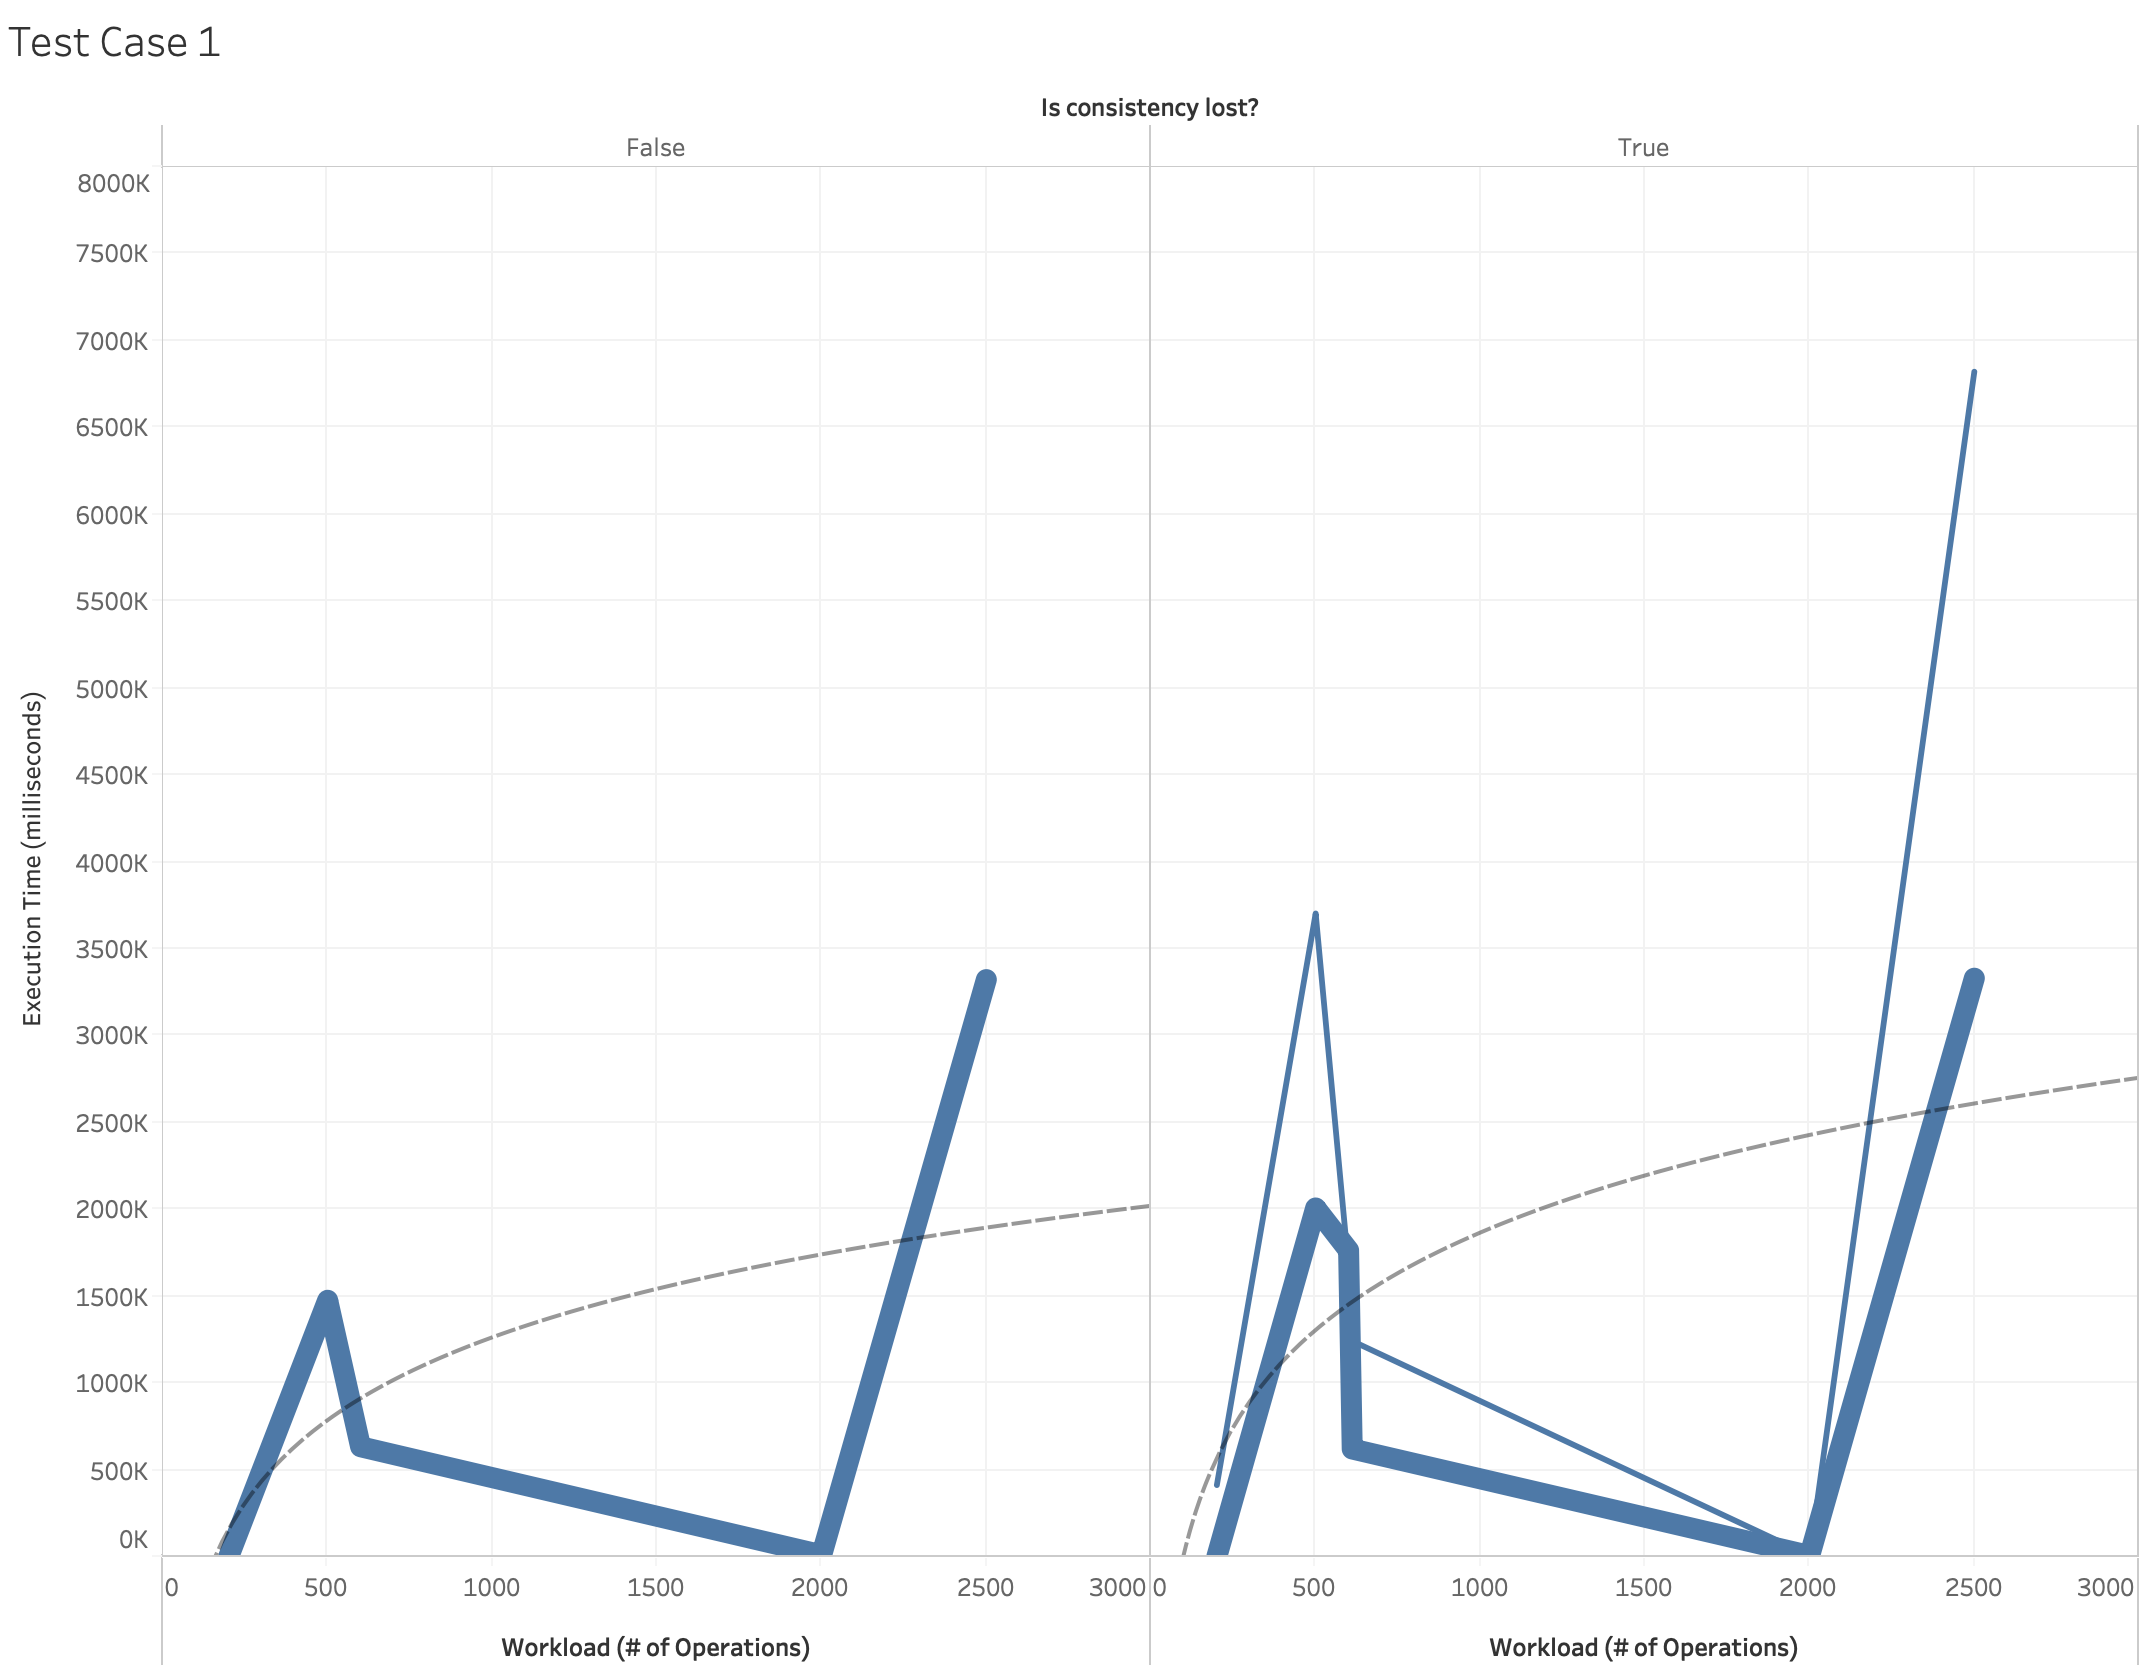
\includegraphics[scale=0.23]{images/TestCase1(WL).png}
\caption{Simulation Results for Test Case 1}
\label{results:test_case_graphs_1}
\end{figure}

\begin{figure}
\centering
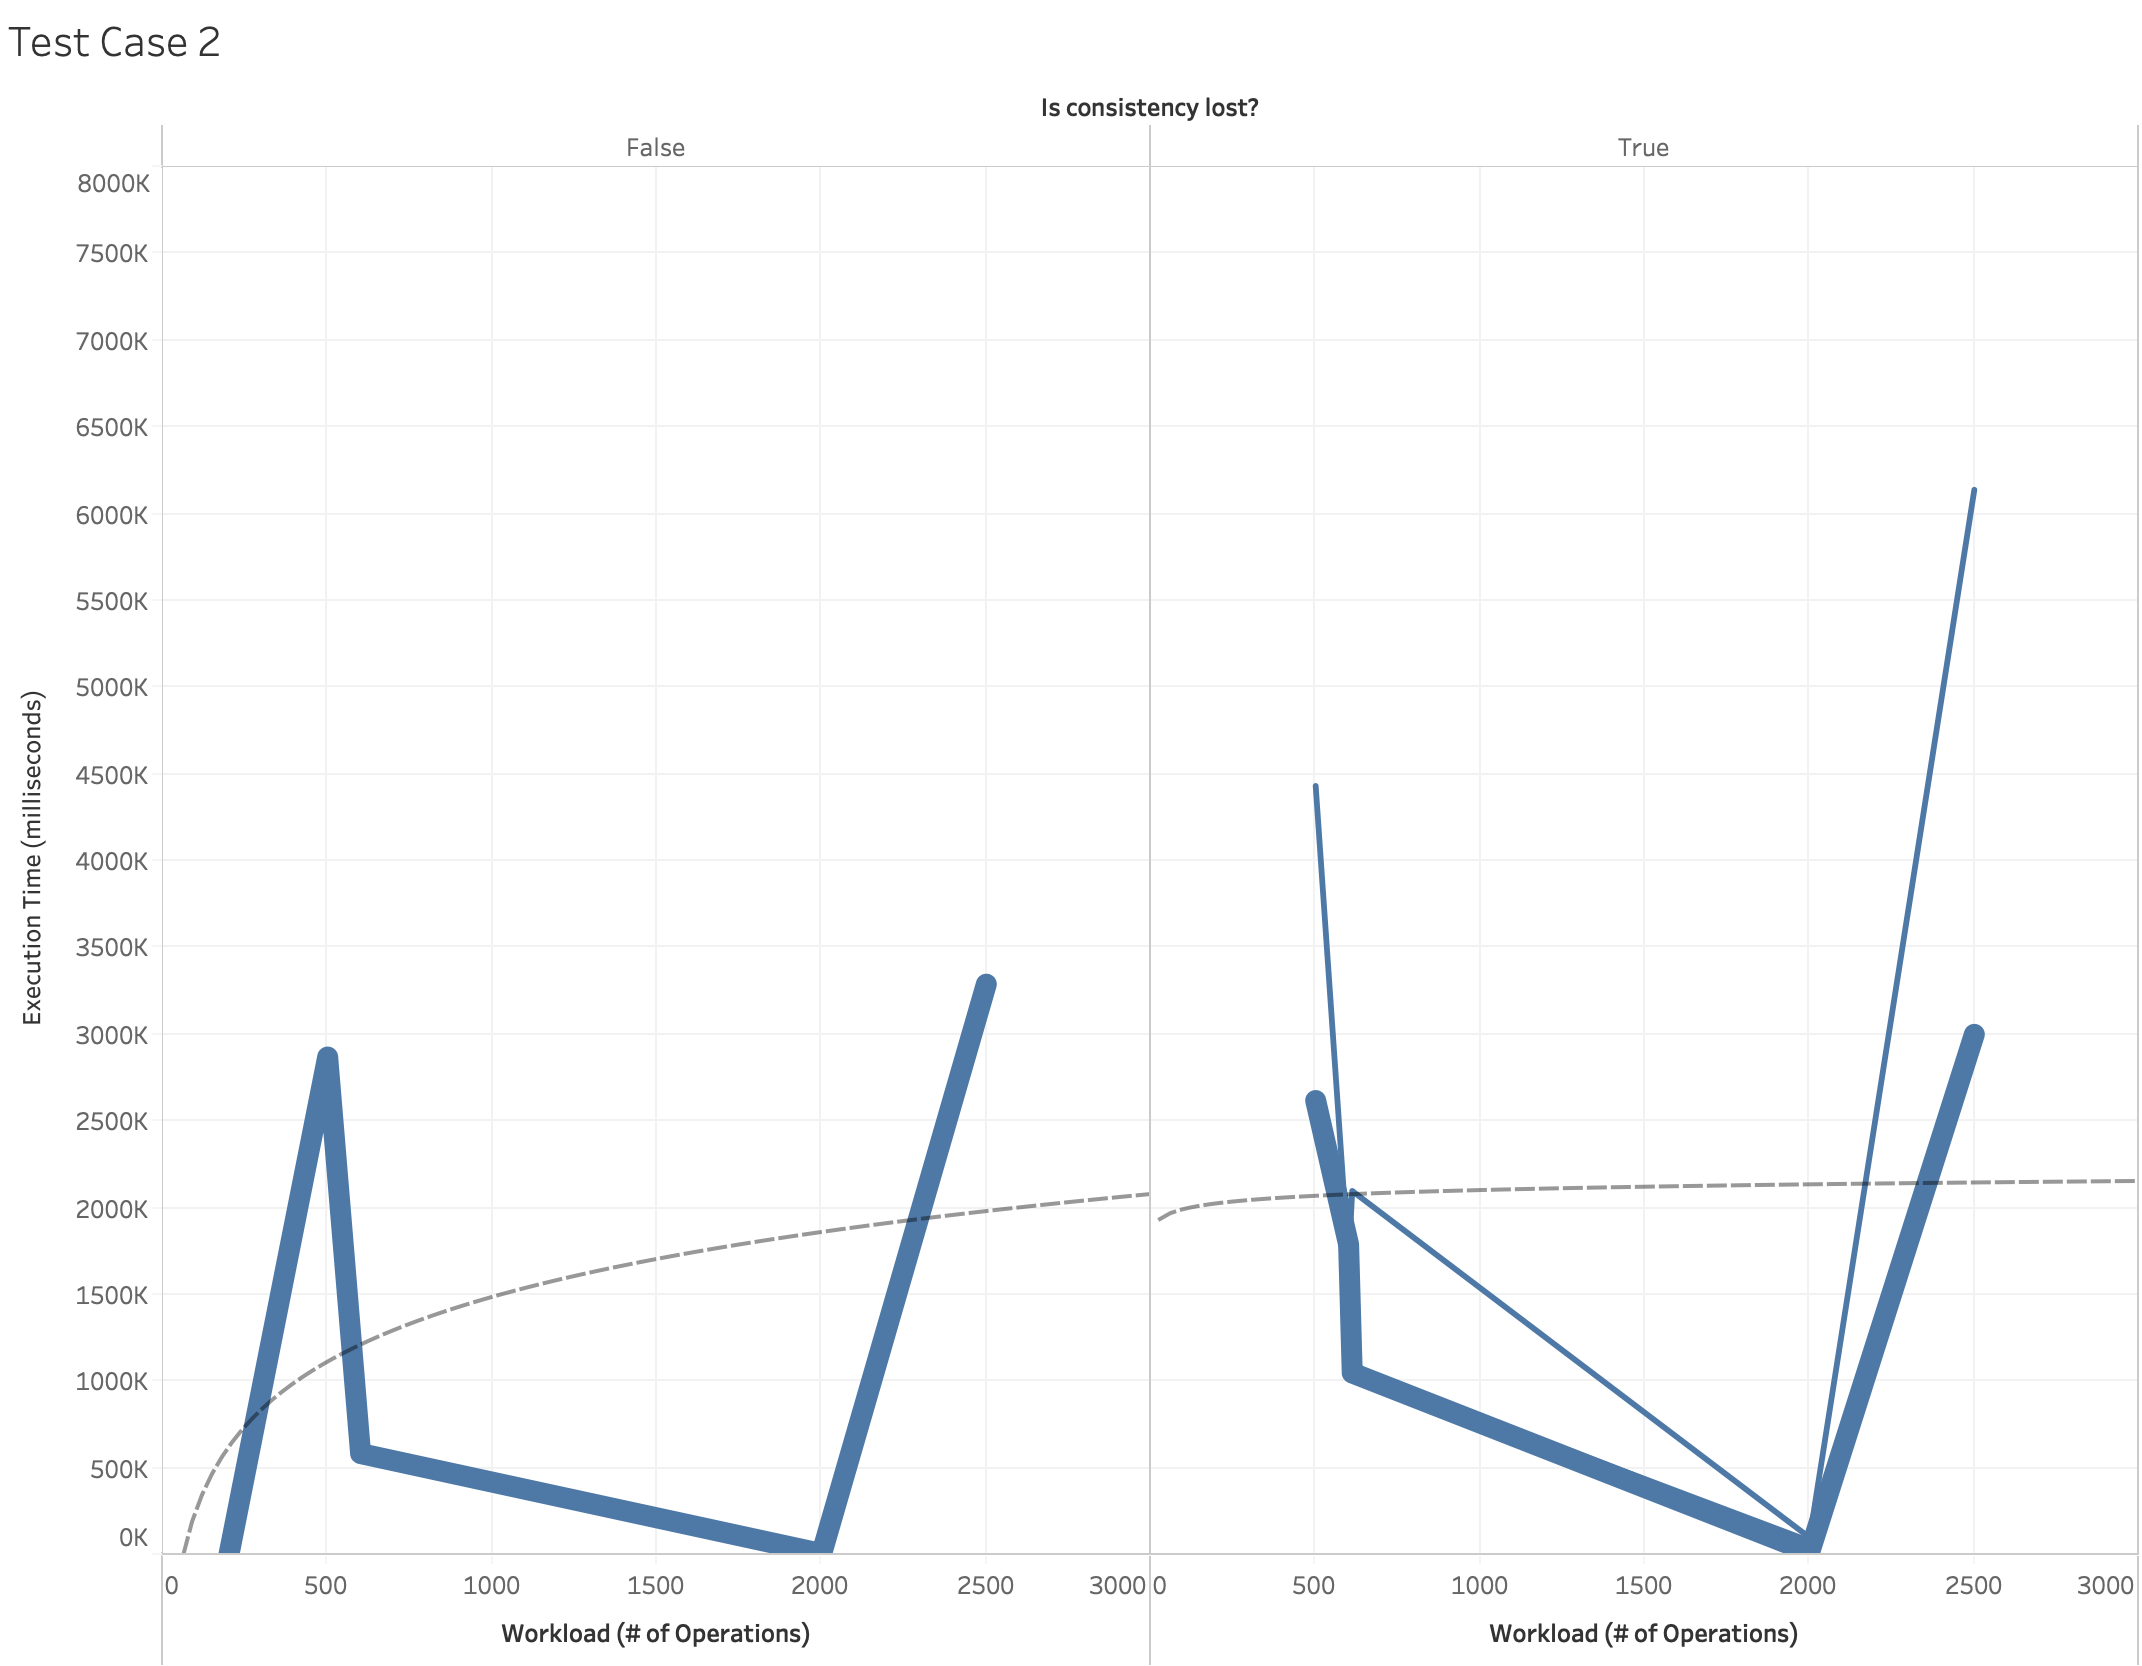
\includegraphics[scale=0.23]{images/TestCase2(WL).png}
\caption{Simulation Results for Test Case 2}
\label{results:test_case_graphs_2}
\end{figure}

\begin{figure}
\centering
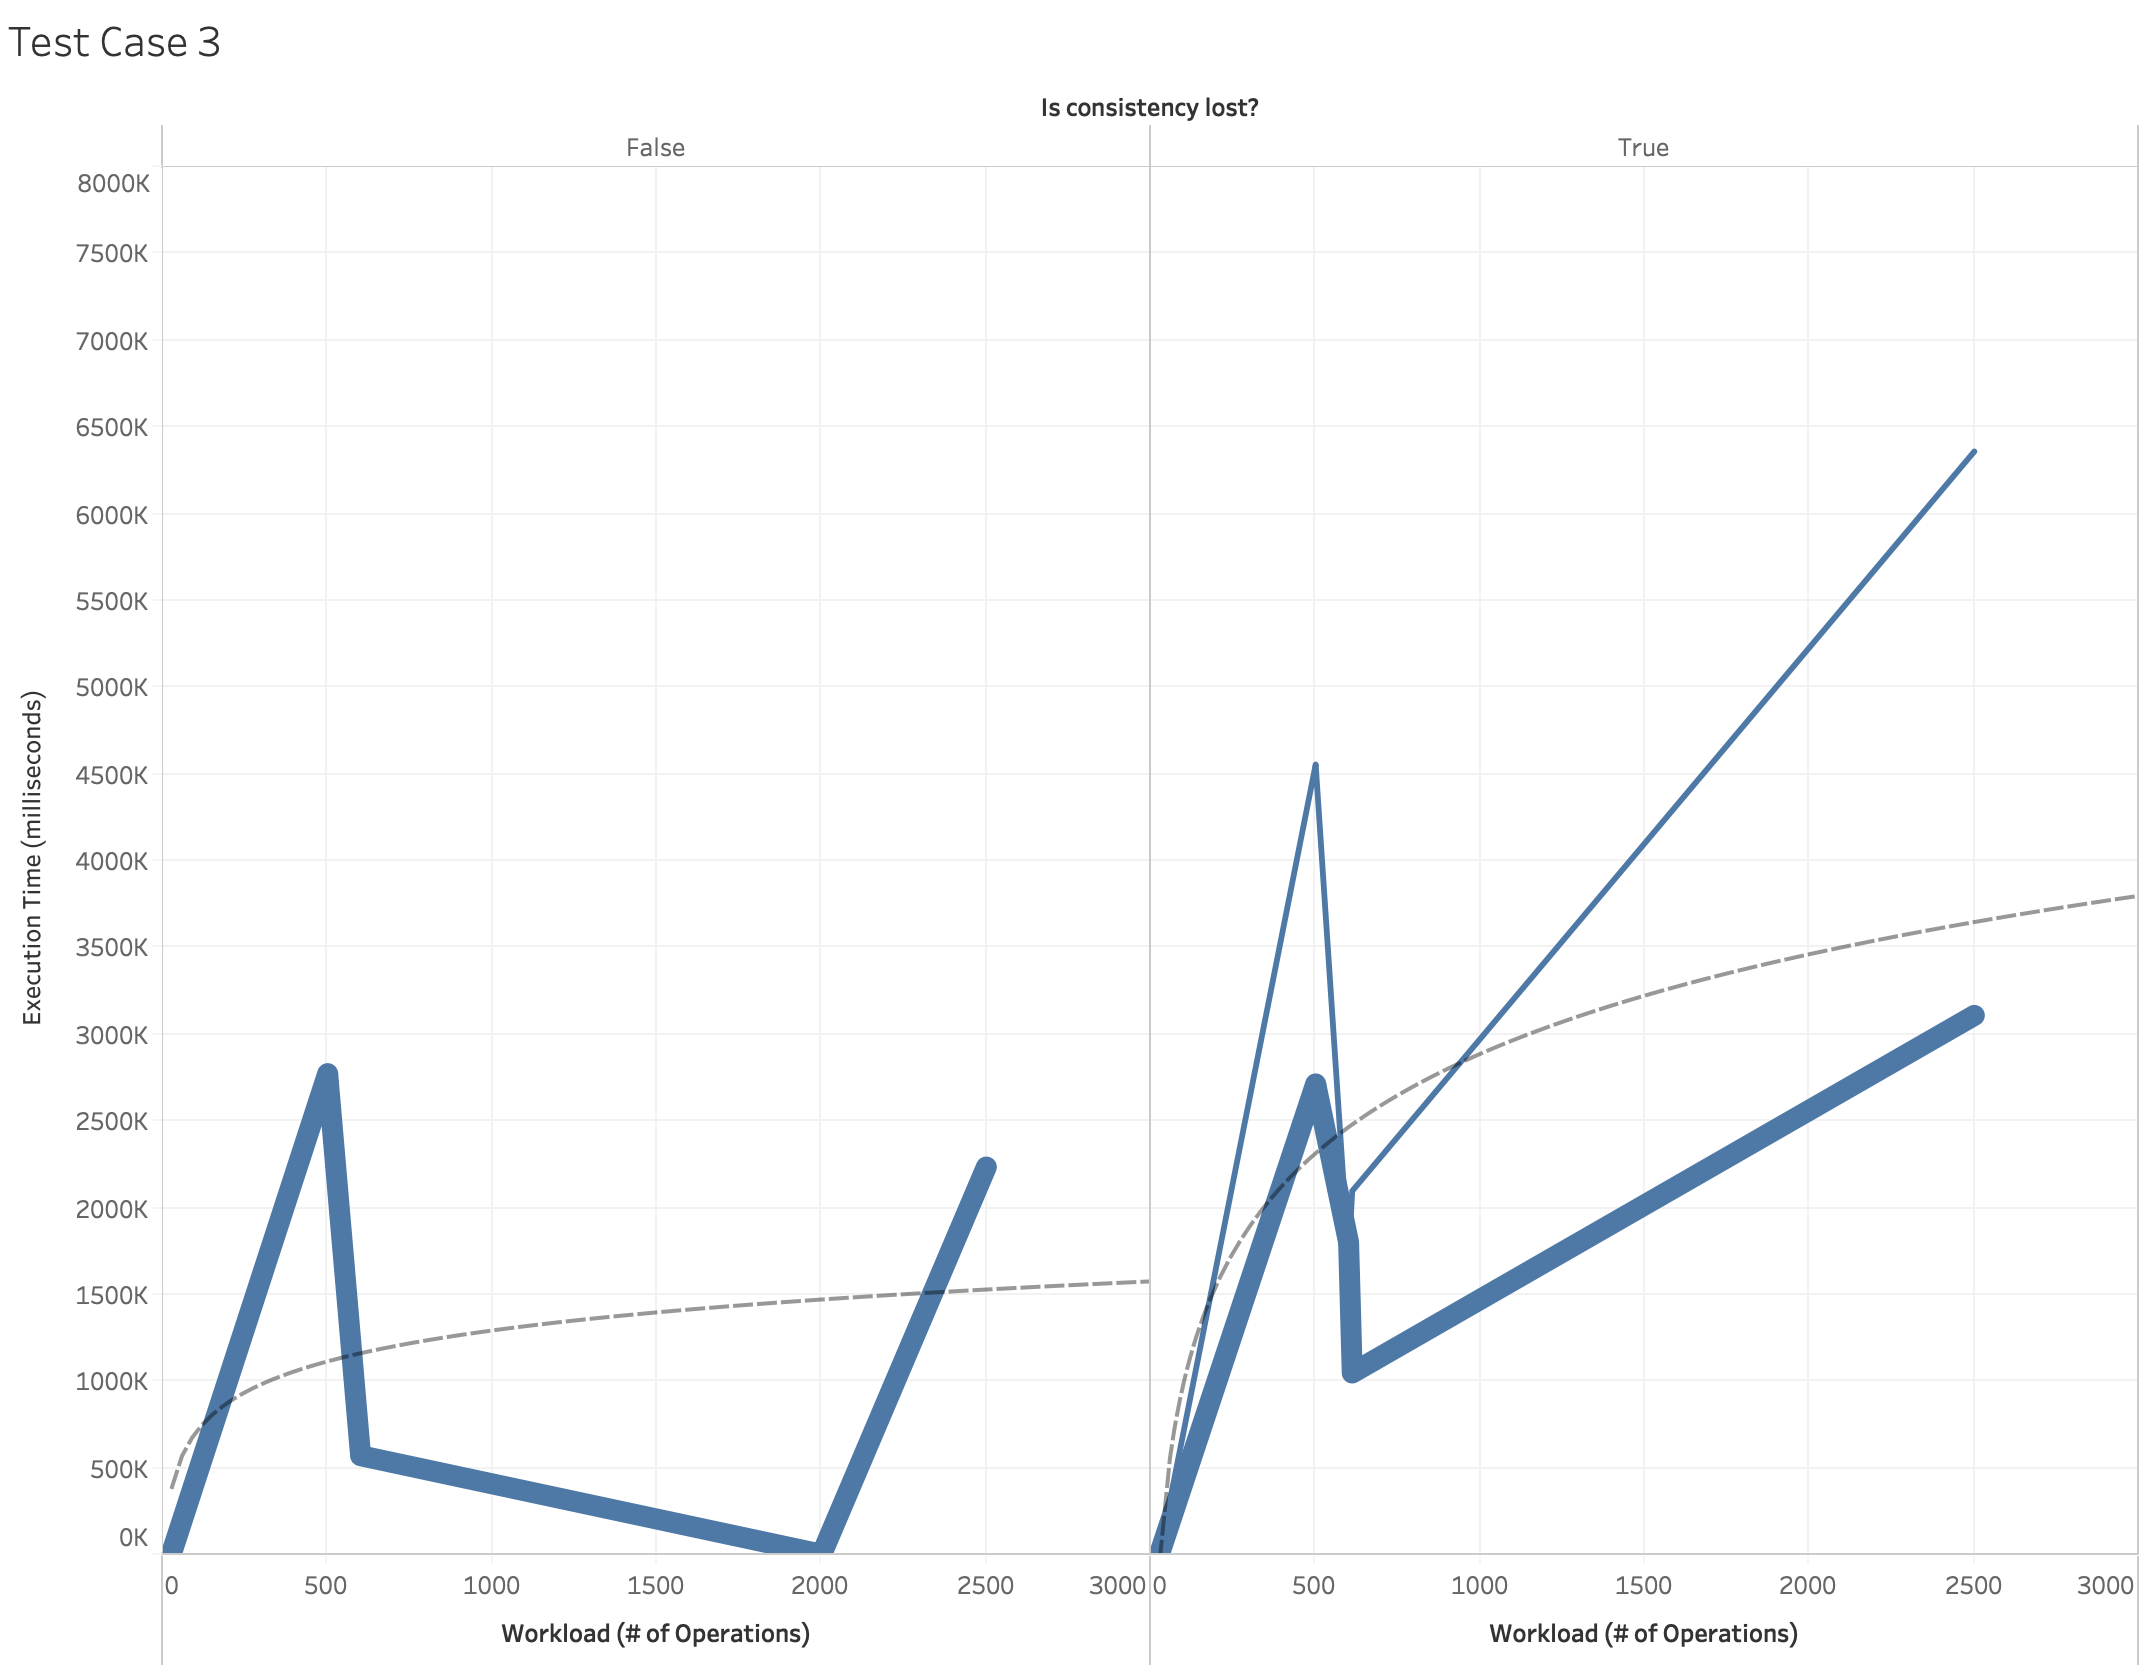
\includegraphics[scale=0.23]{images/TestCase3(WL).png}
\caption{Simulation Results for Test Case 3}
\label{results:test_case_graphs_3}
\end{figure}

\begin{figure}
\centering
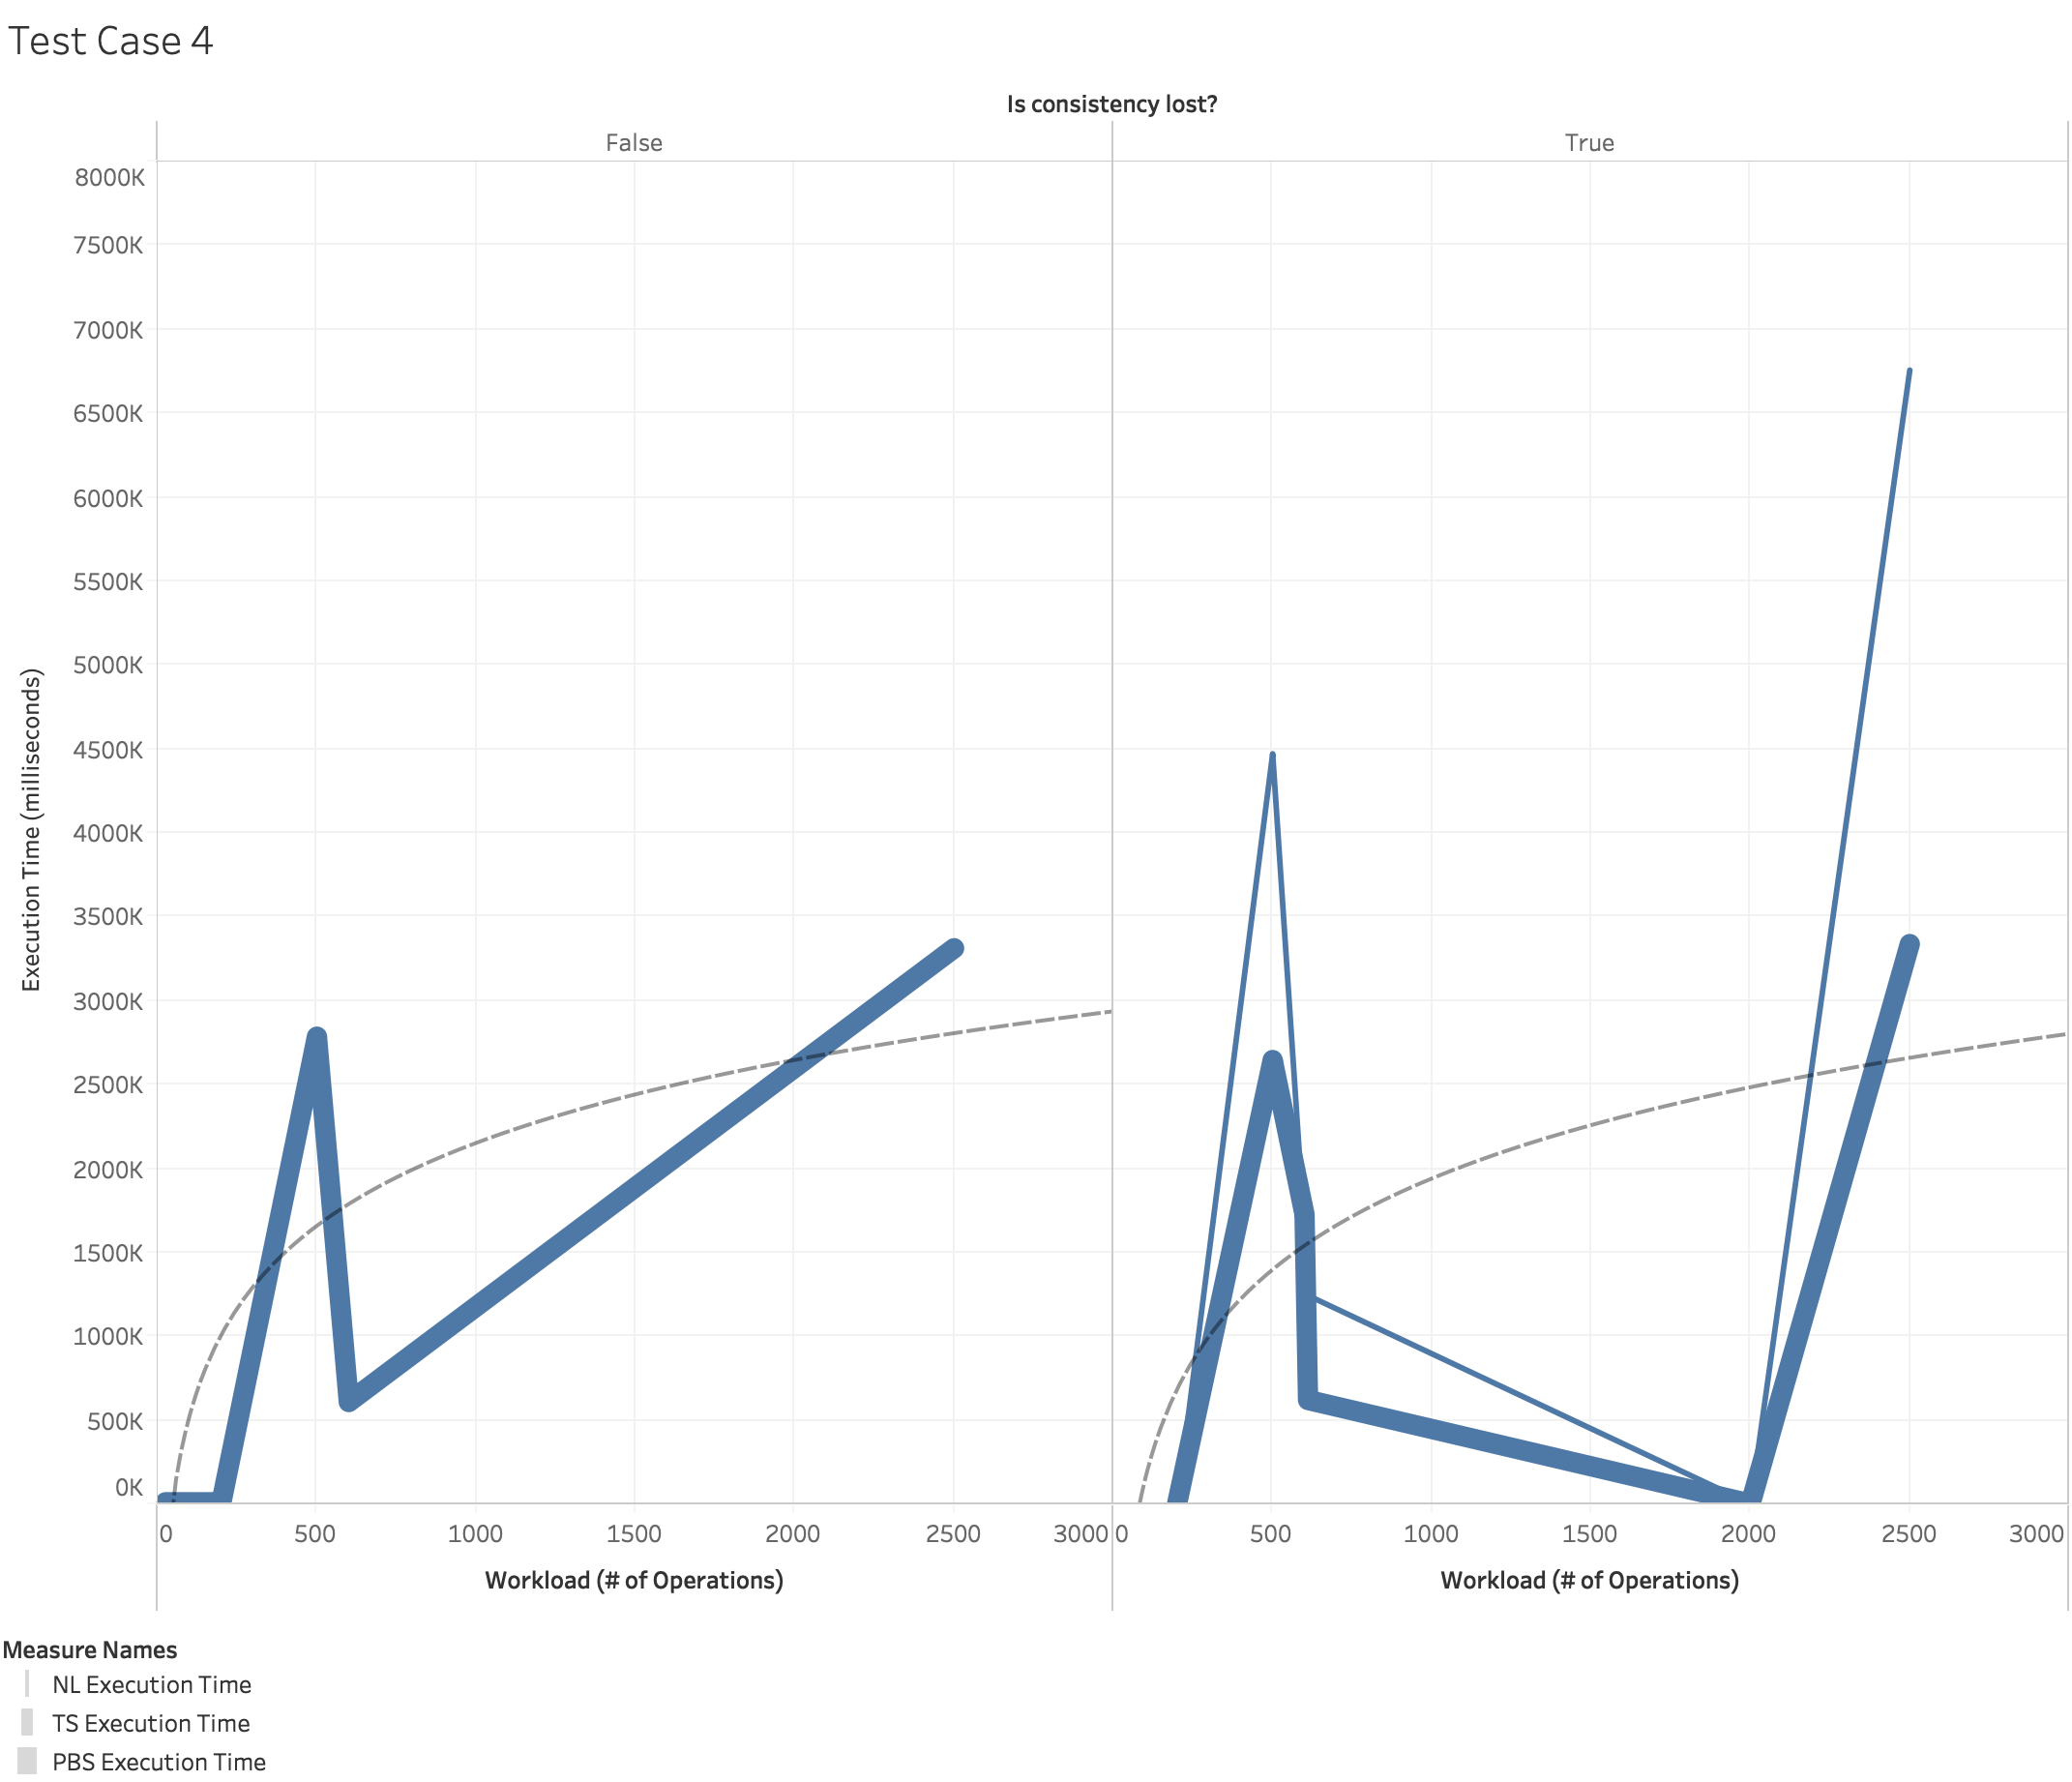
\includegraphics[scale=0.23]{images/TestCase4(WL).png}
\caption{Simulation Results for Test Case 4}
\label{results:test_case_graphs_4}
\end{figure}

\begin{figure}
\centering
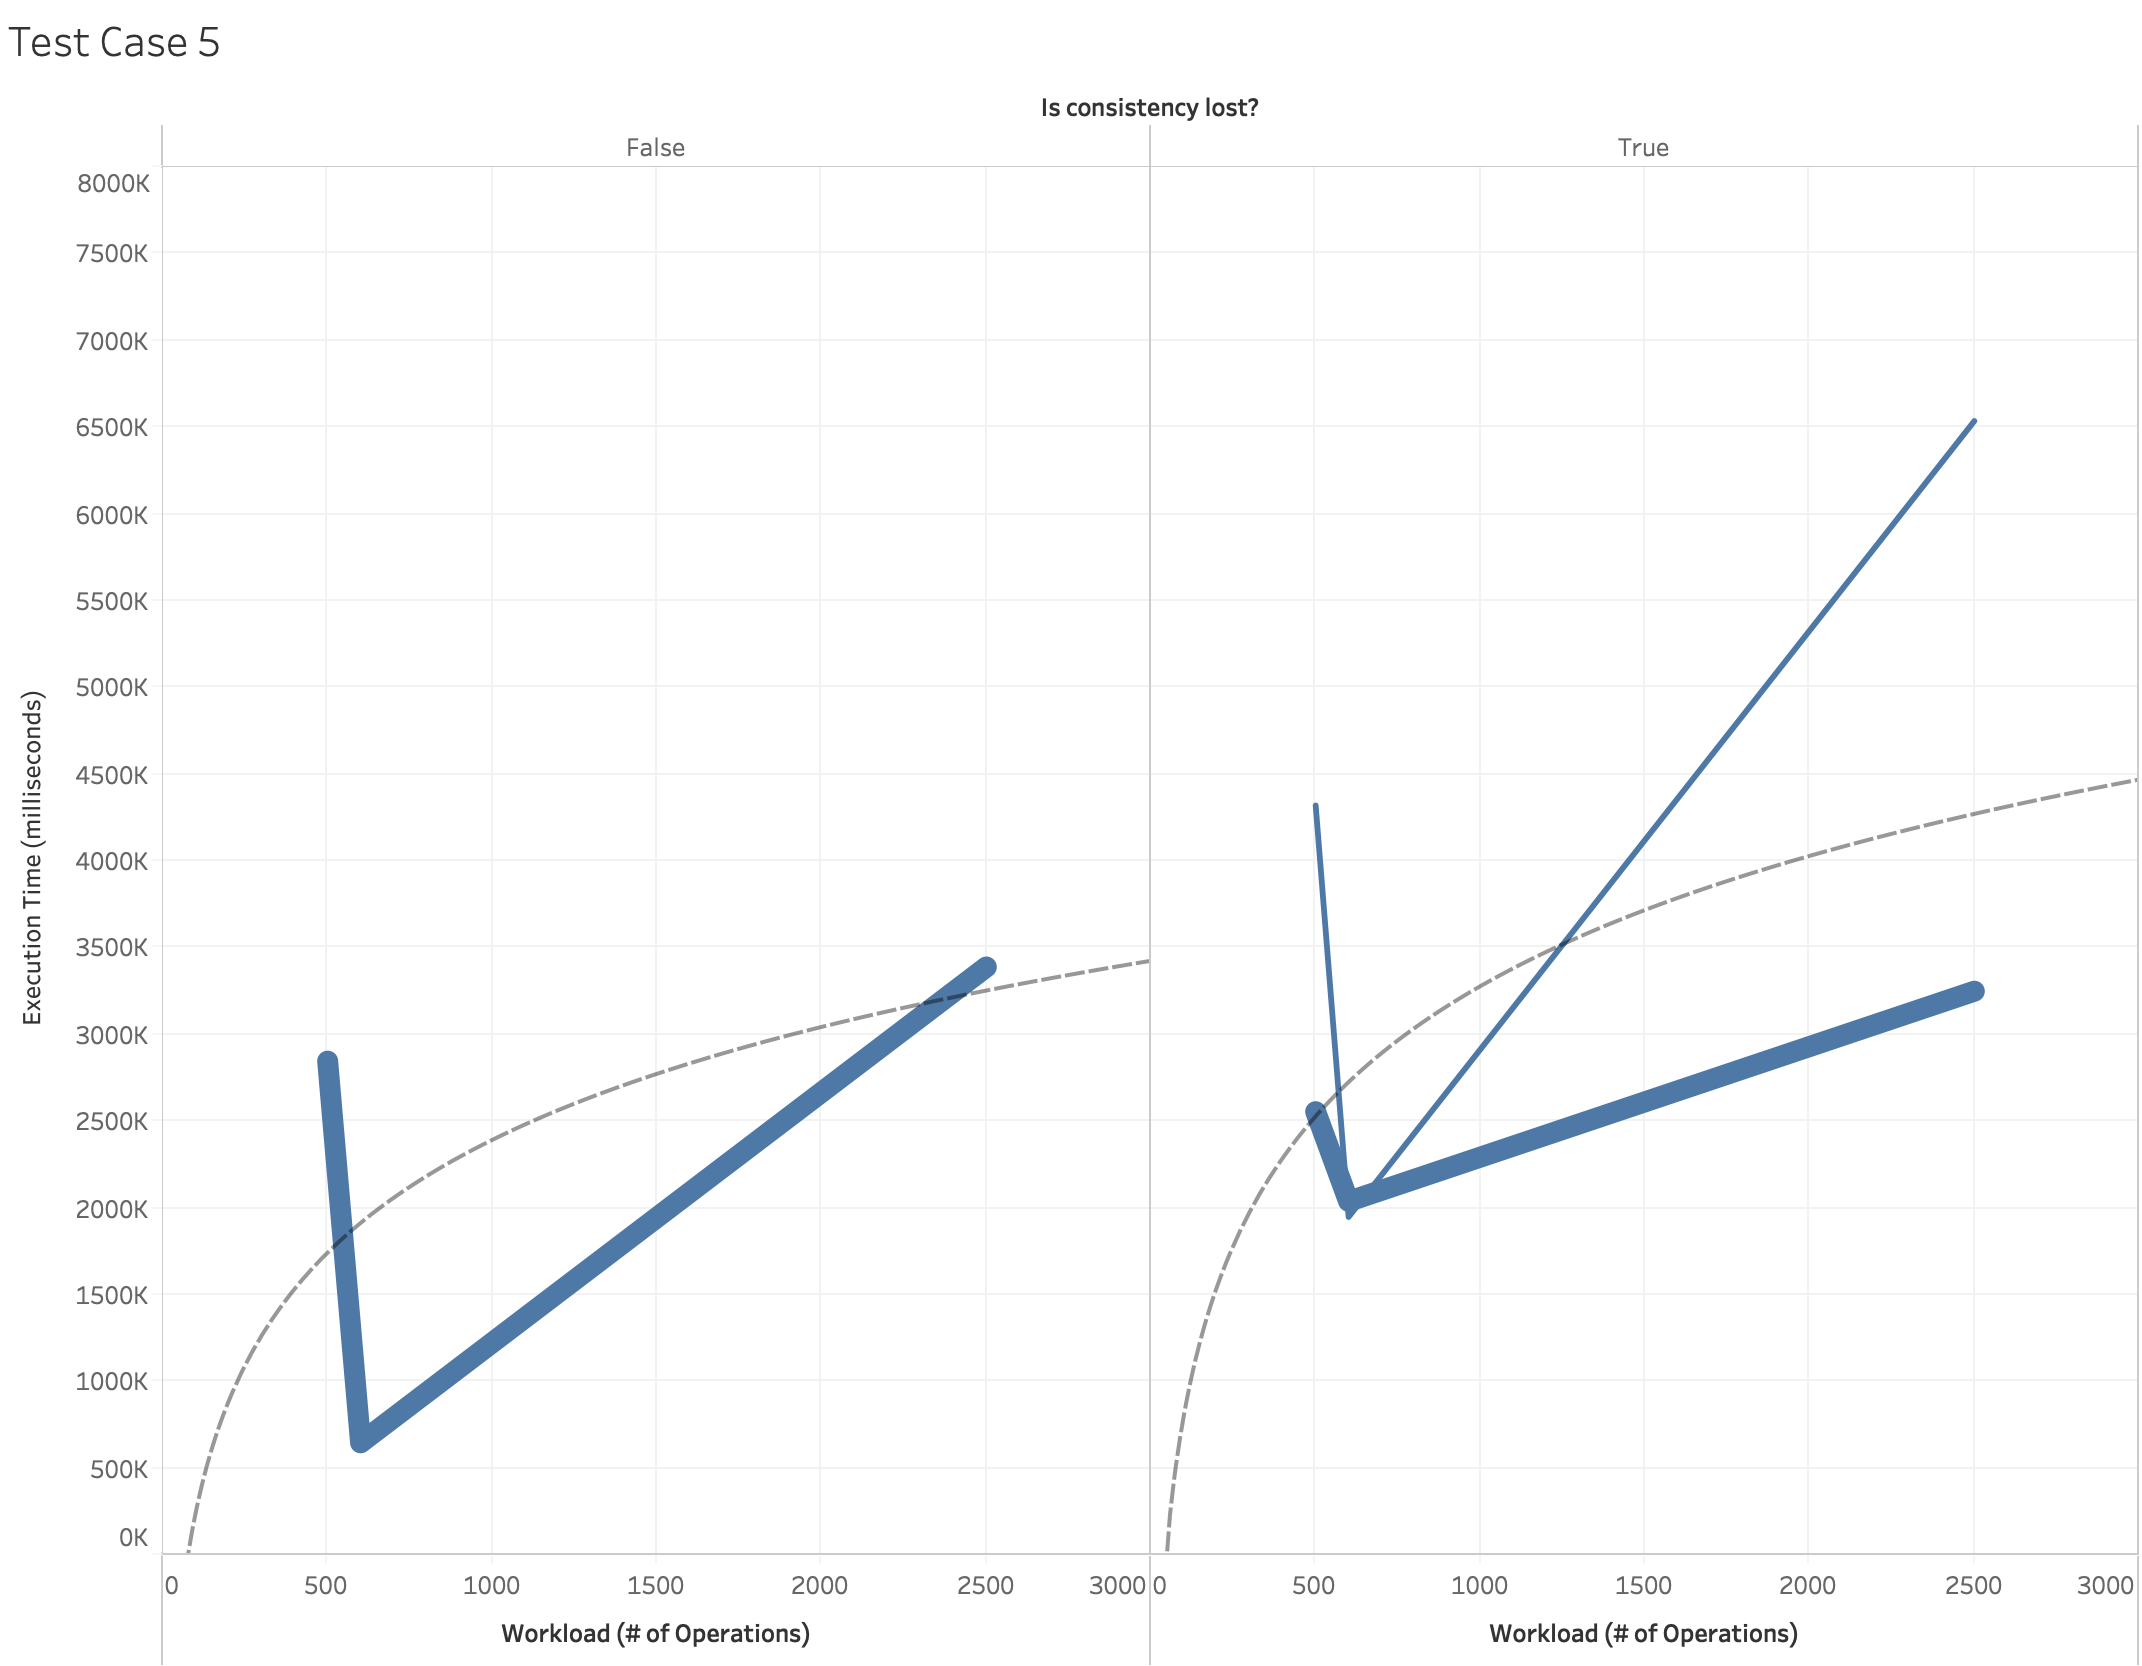
\includegraphics[scale=0.23]{images/TestCase5(WL).png}
\caption{Simulation Results for Test Case 5}
\label{results:test_case_graphs_5}
\end{figure}

\begin{figure}
\centering
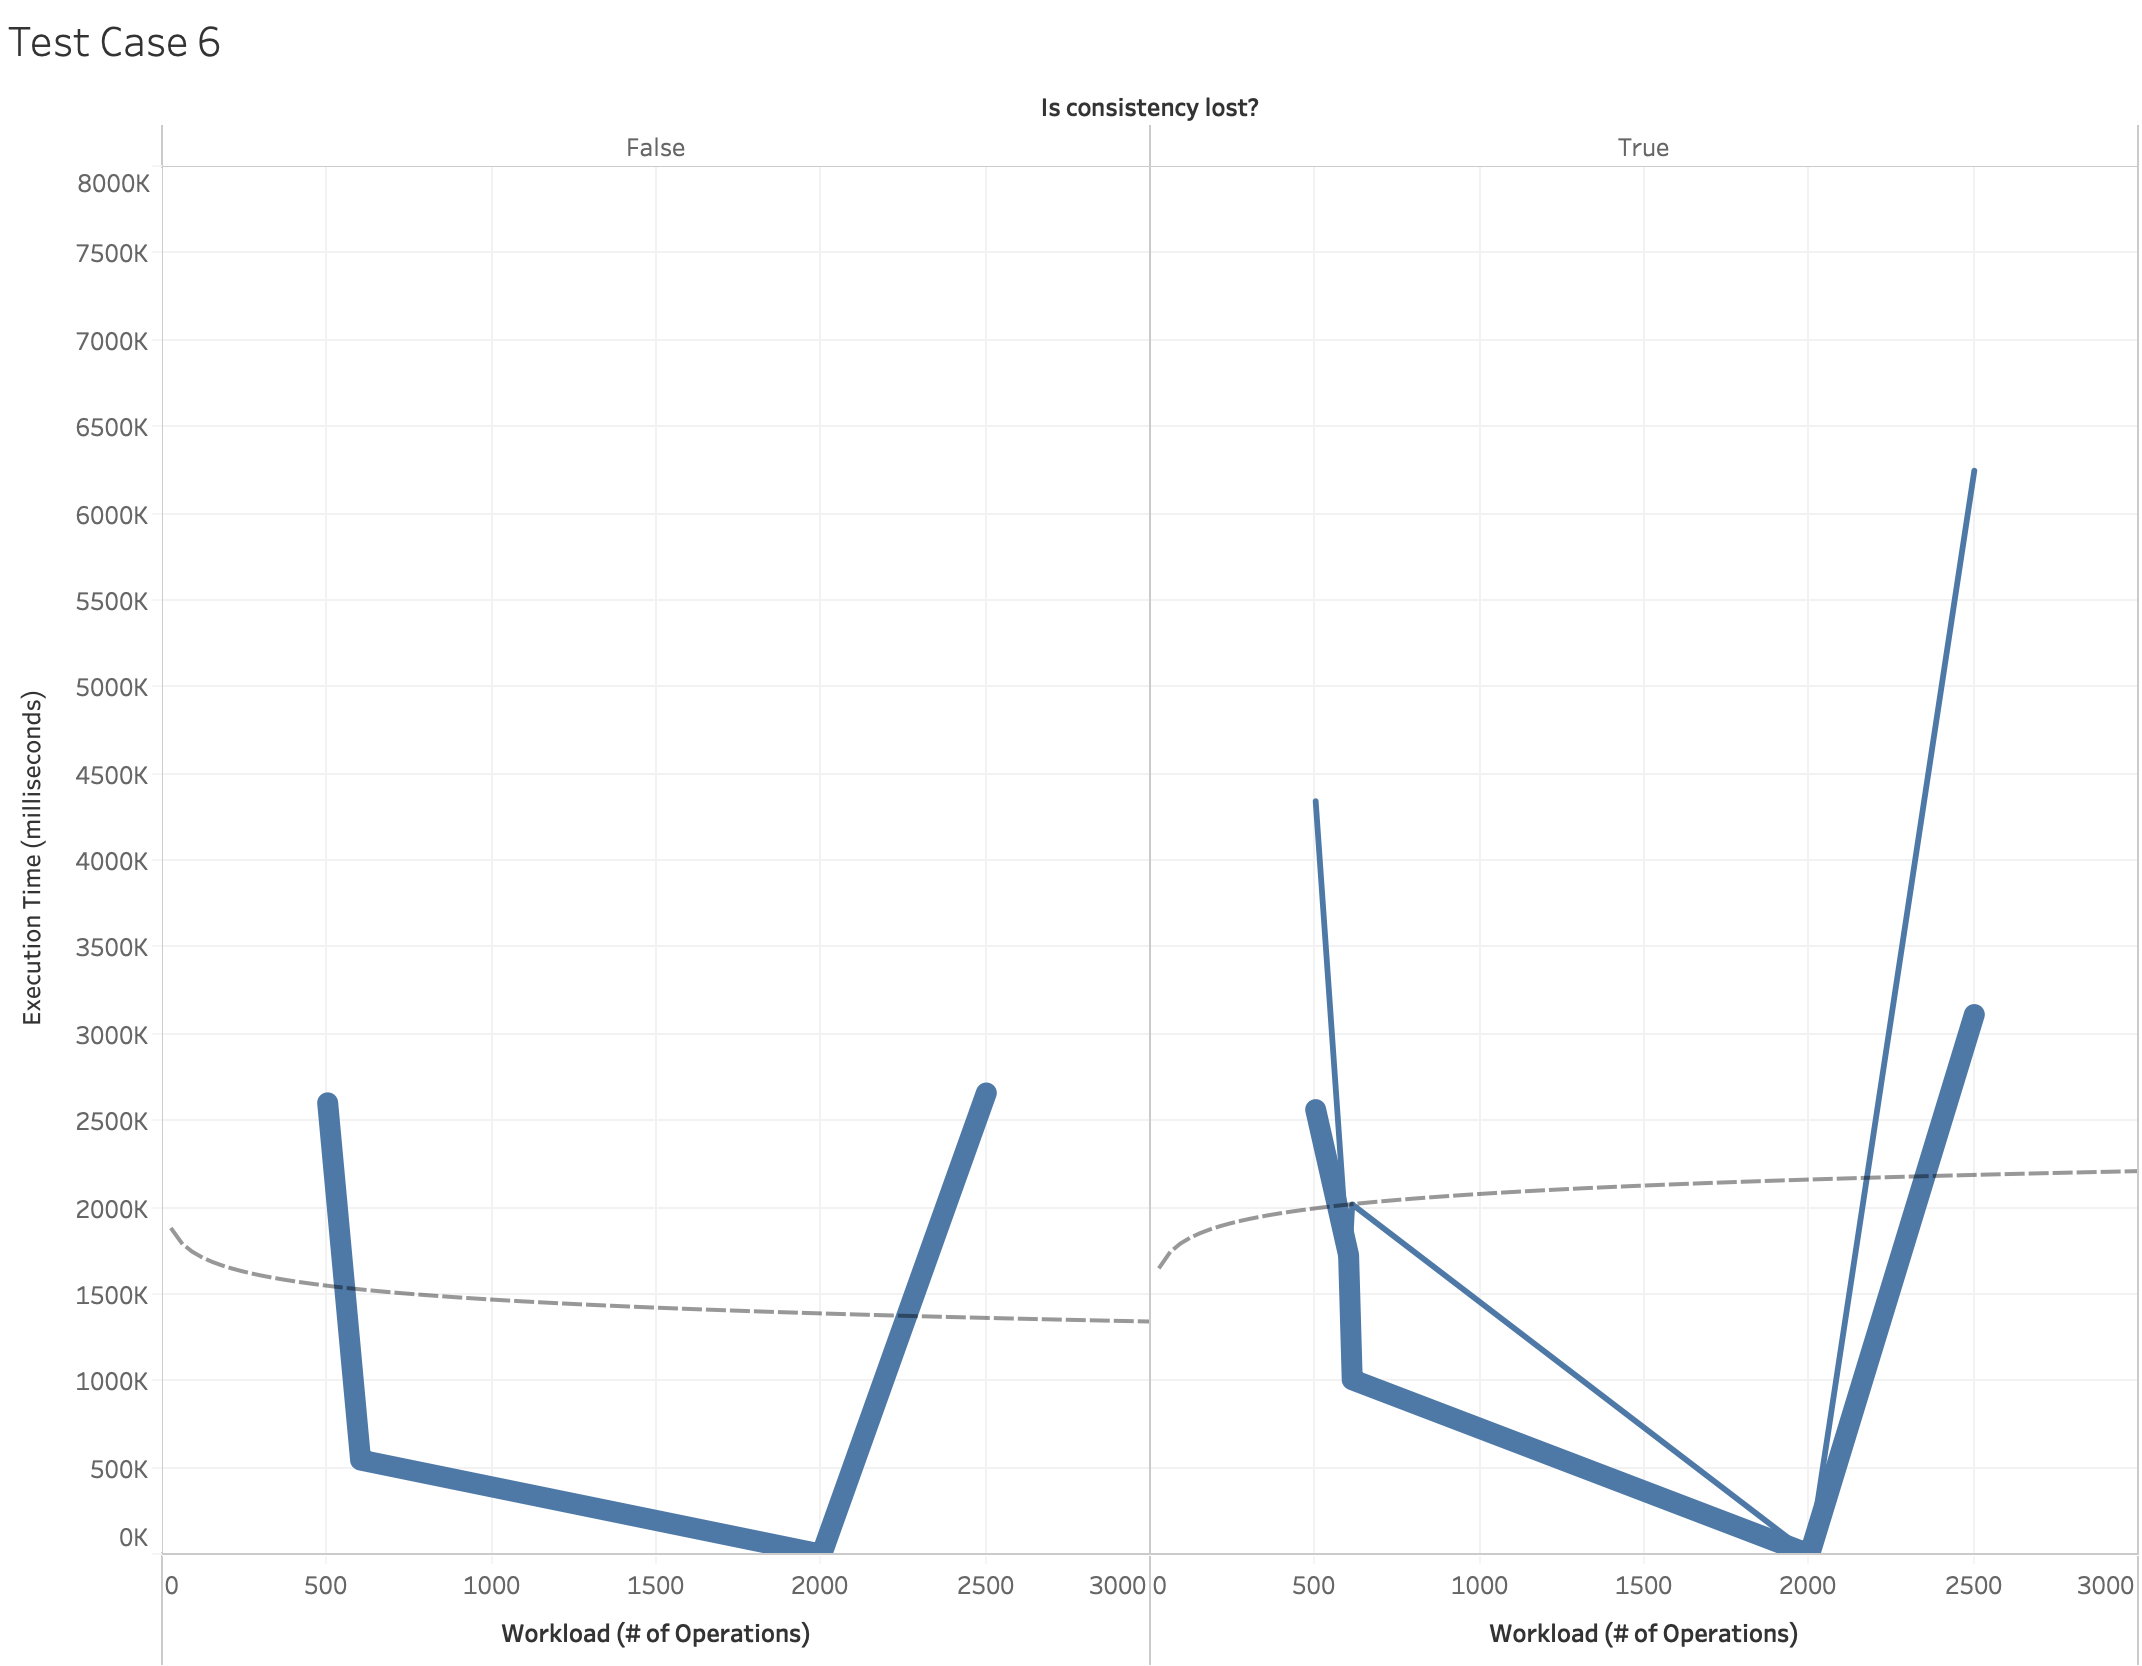
\includegraphics[scale=0.20]{images/TestCase6(WL).png}
\caption{Simulation Results for Test Case 6}
\label{results:test_case_graphs_6}
\end{figure}

\begin{figure}
\centering
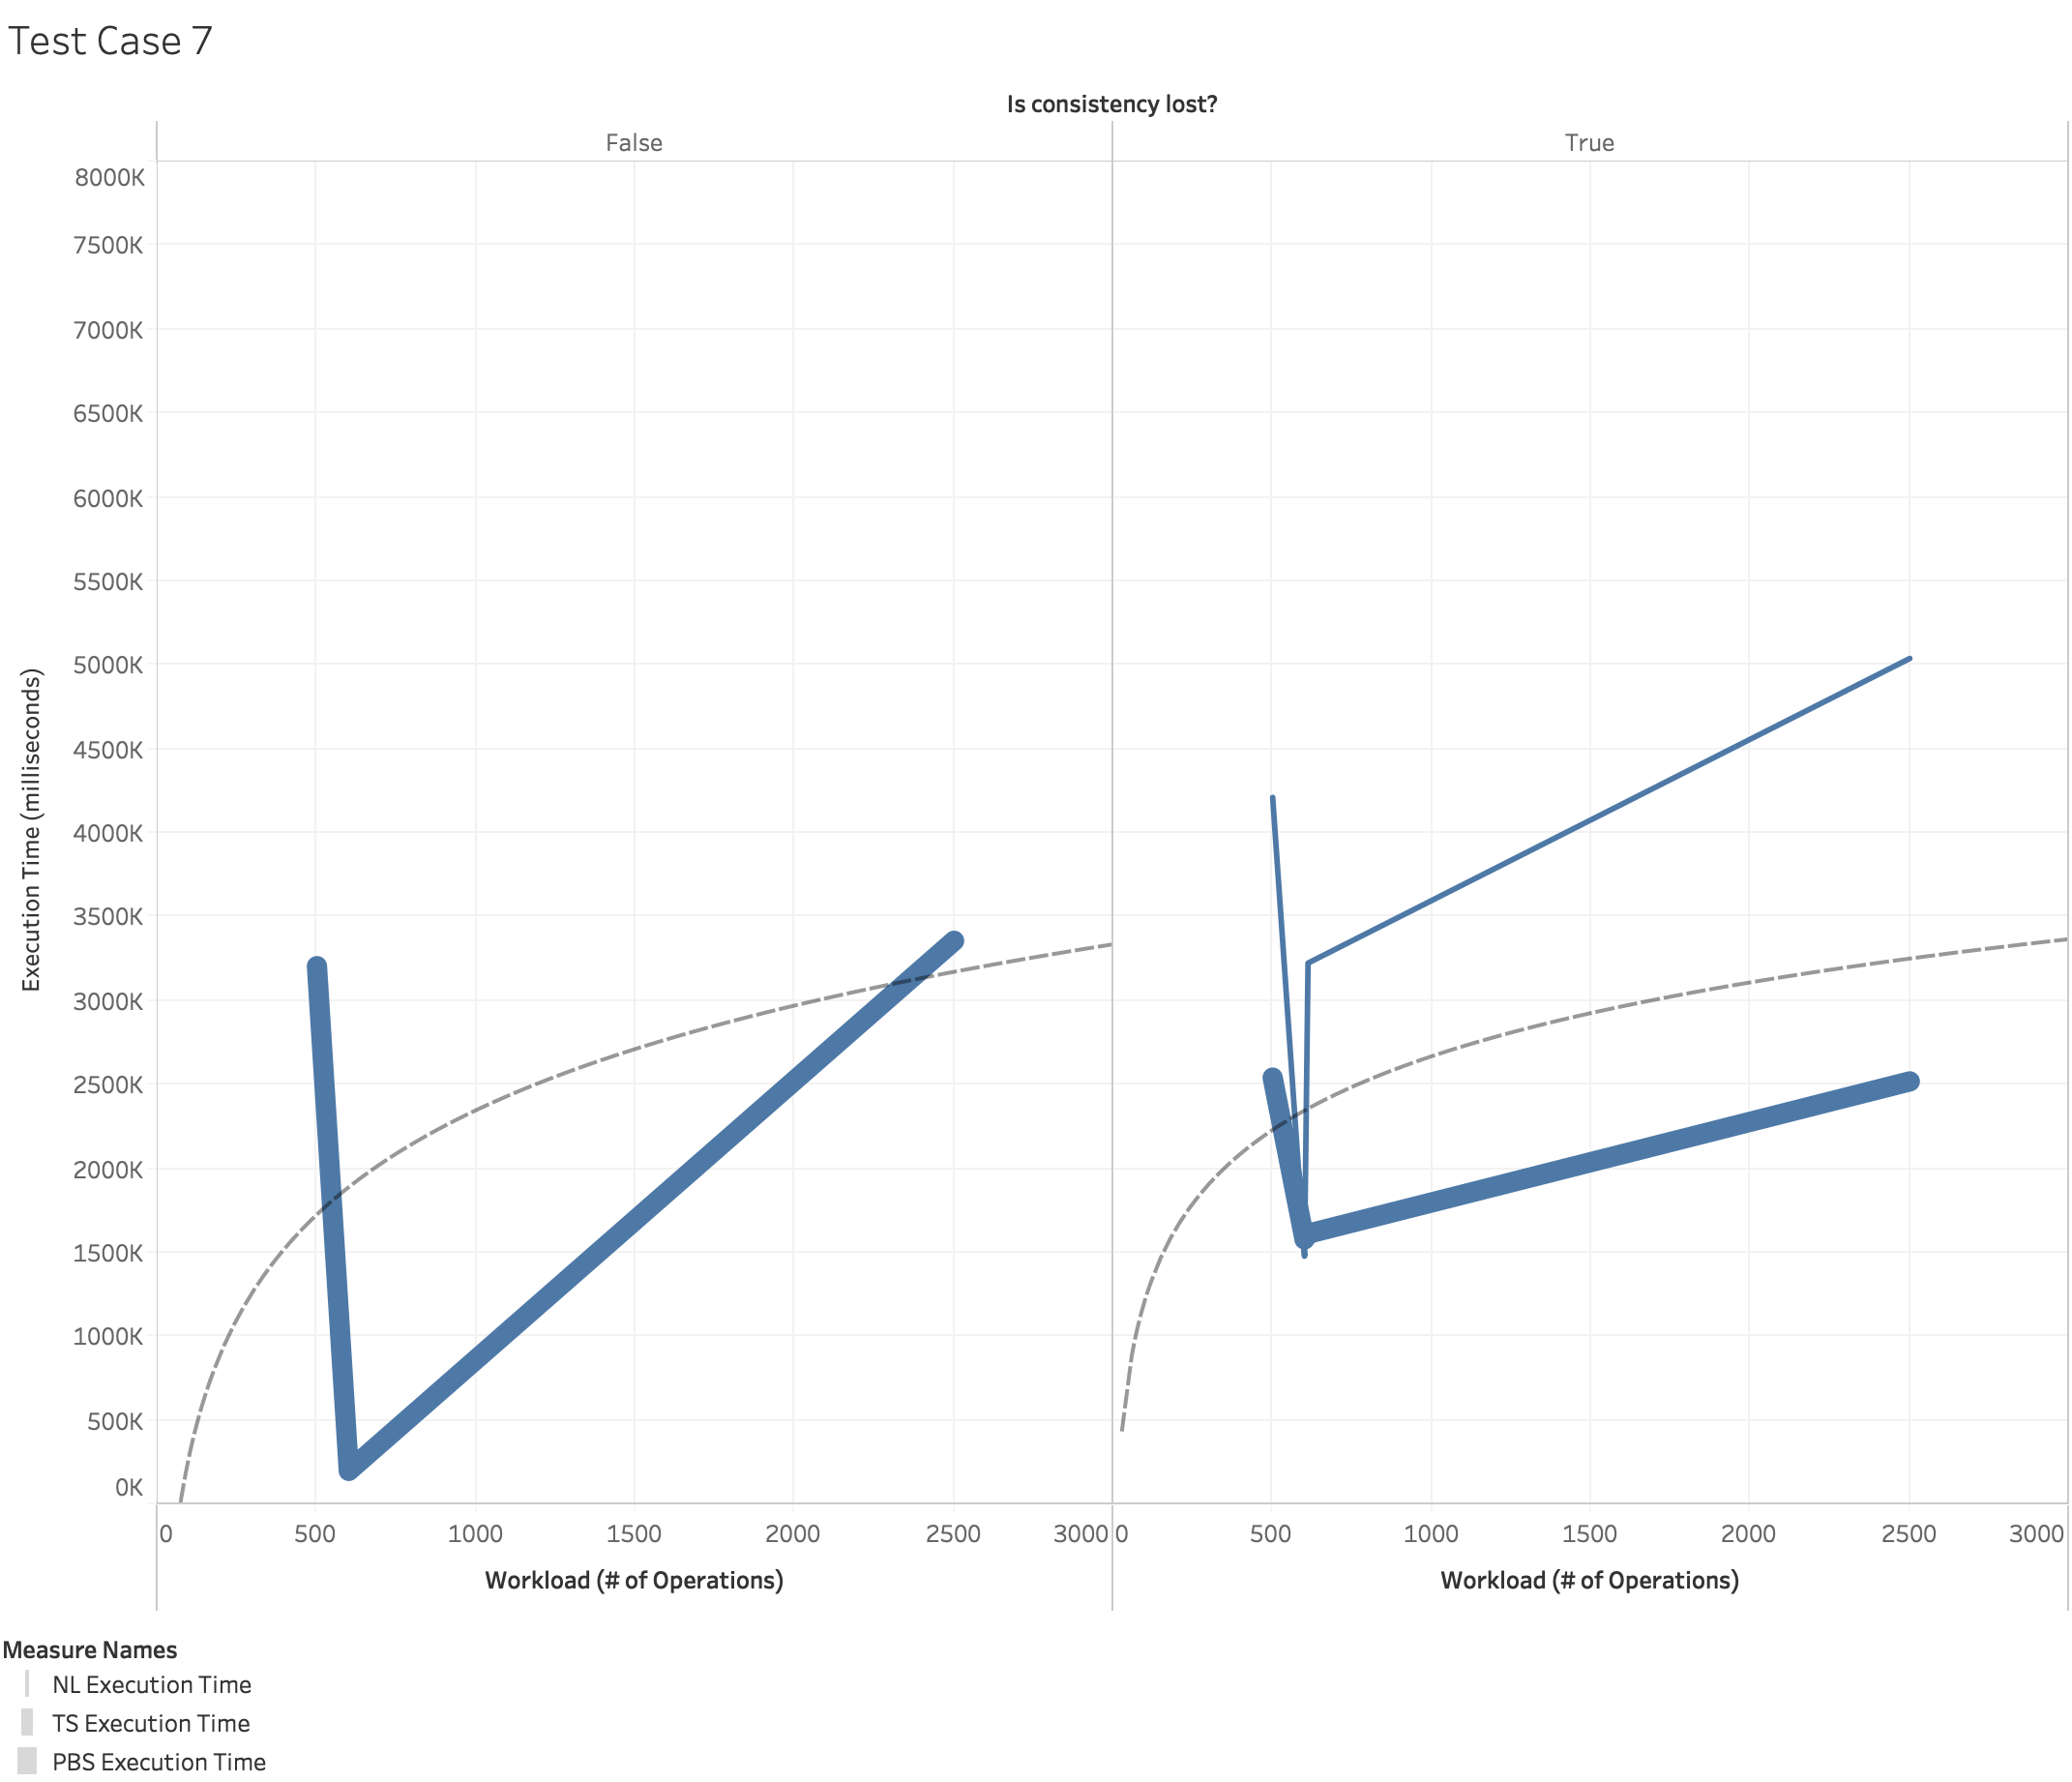
\includegraphics[scale=0.20]{images/TestCase7(WL).png}
\caption{Simulation Results for Test Case 7}
\label{results:test_case_graphs_7}
\end{figure}

\begin{figure}
\centering
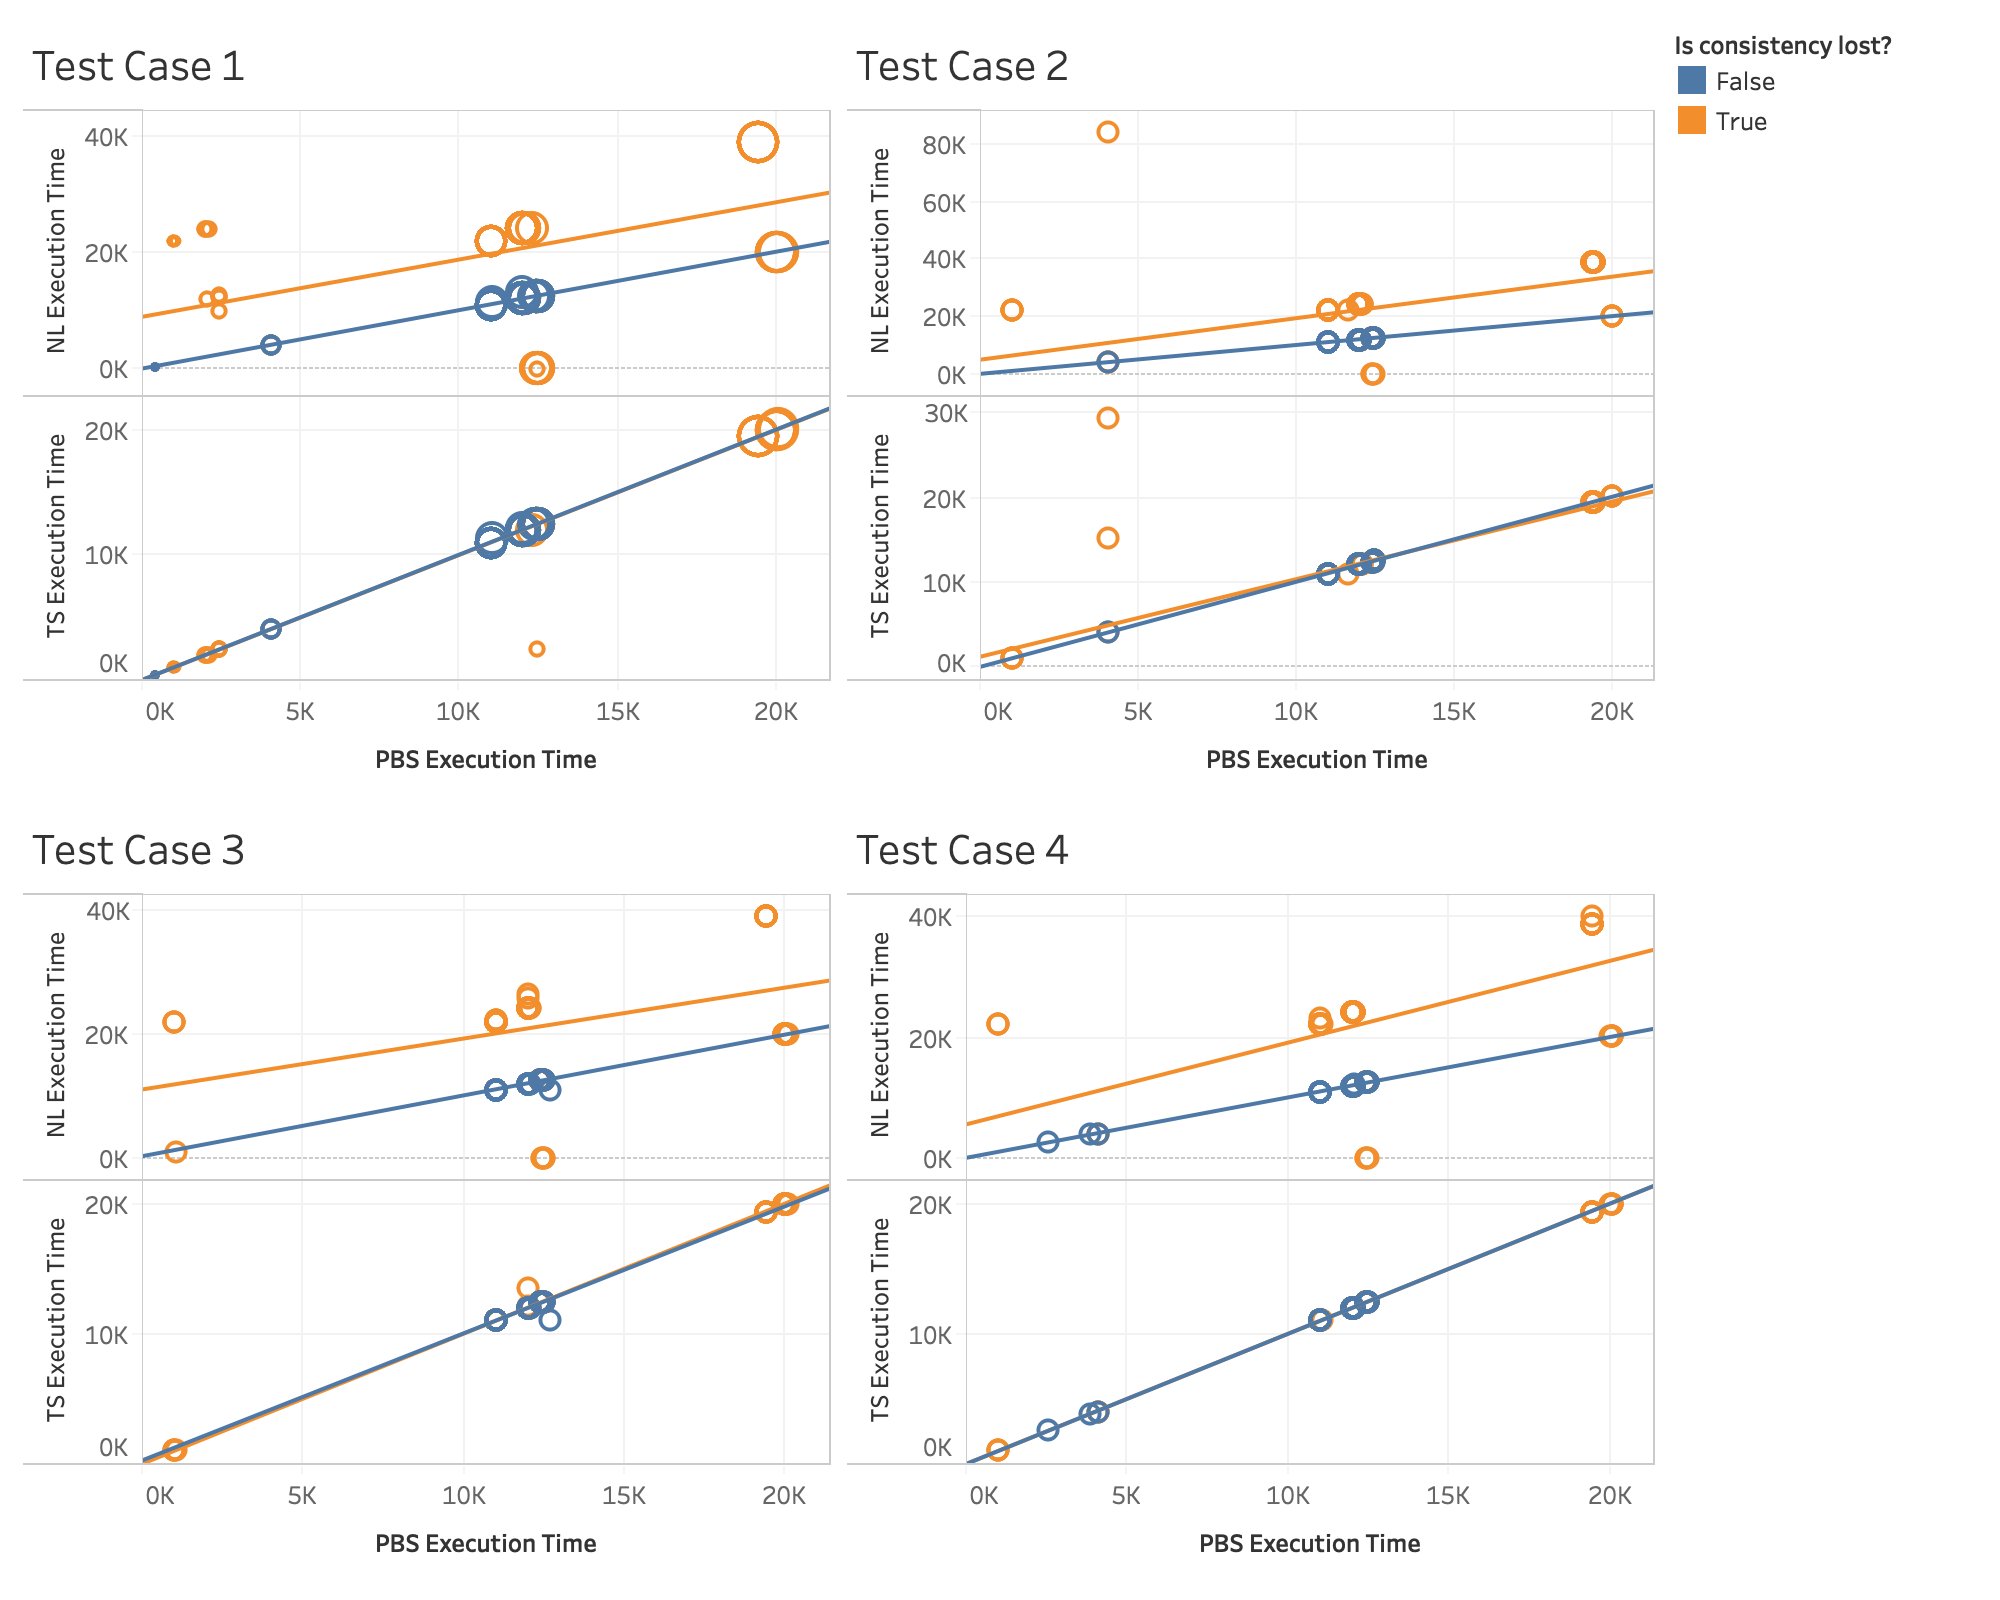
\includegraphics[scale=0.25]{images/Dashboard1_TL.png}
\caption{Consistency Lost/Kept for Test Cases 1-4}
\label{results:consistency_test_case_graphs_1_4}
\end{figure}

\begin{figure}
\centering
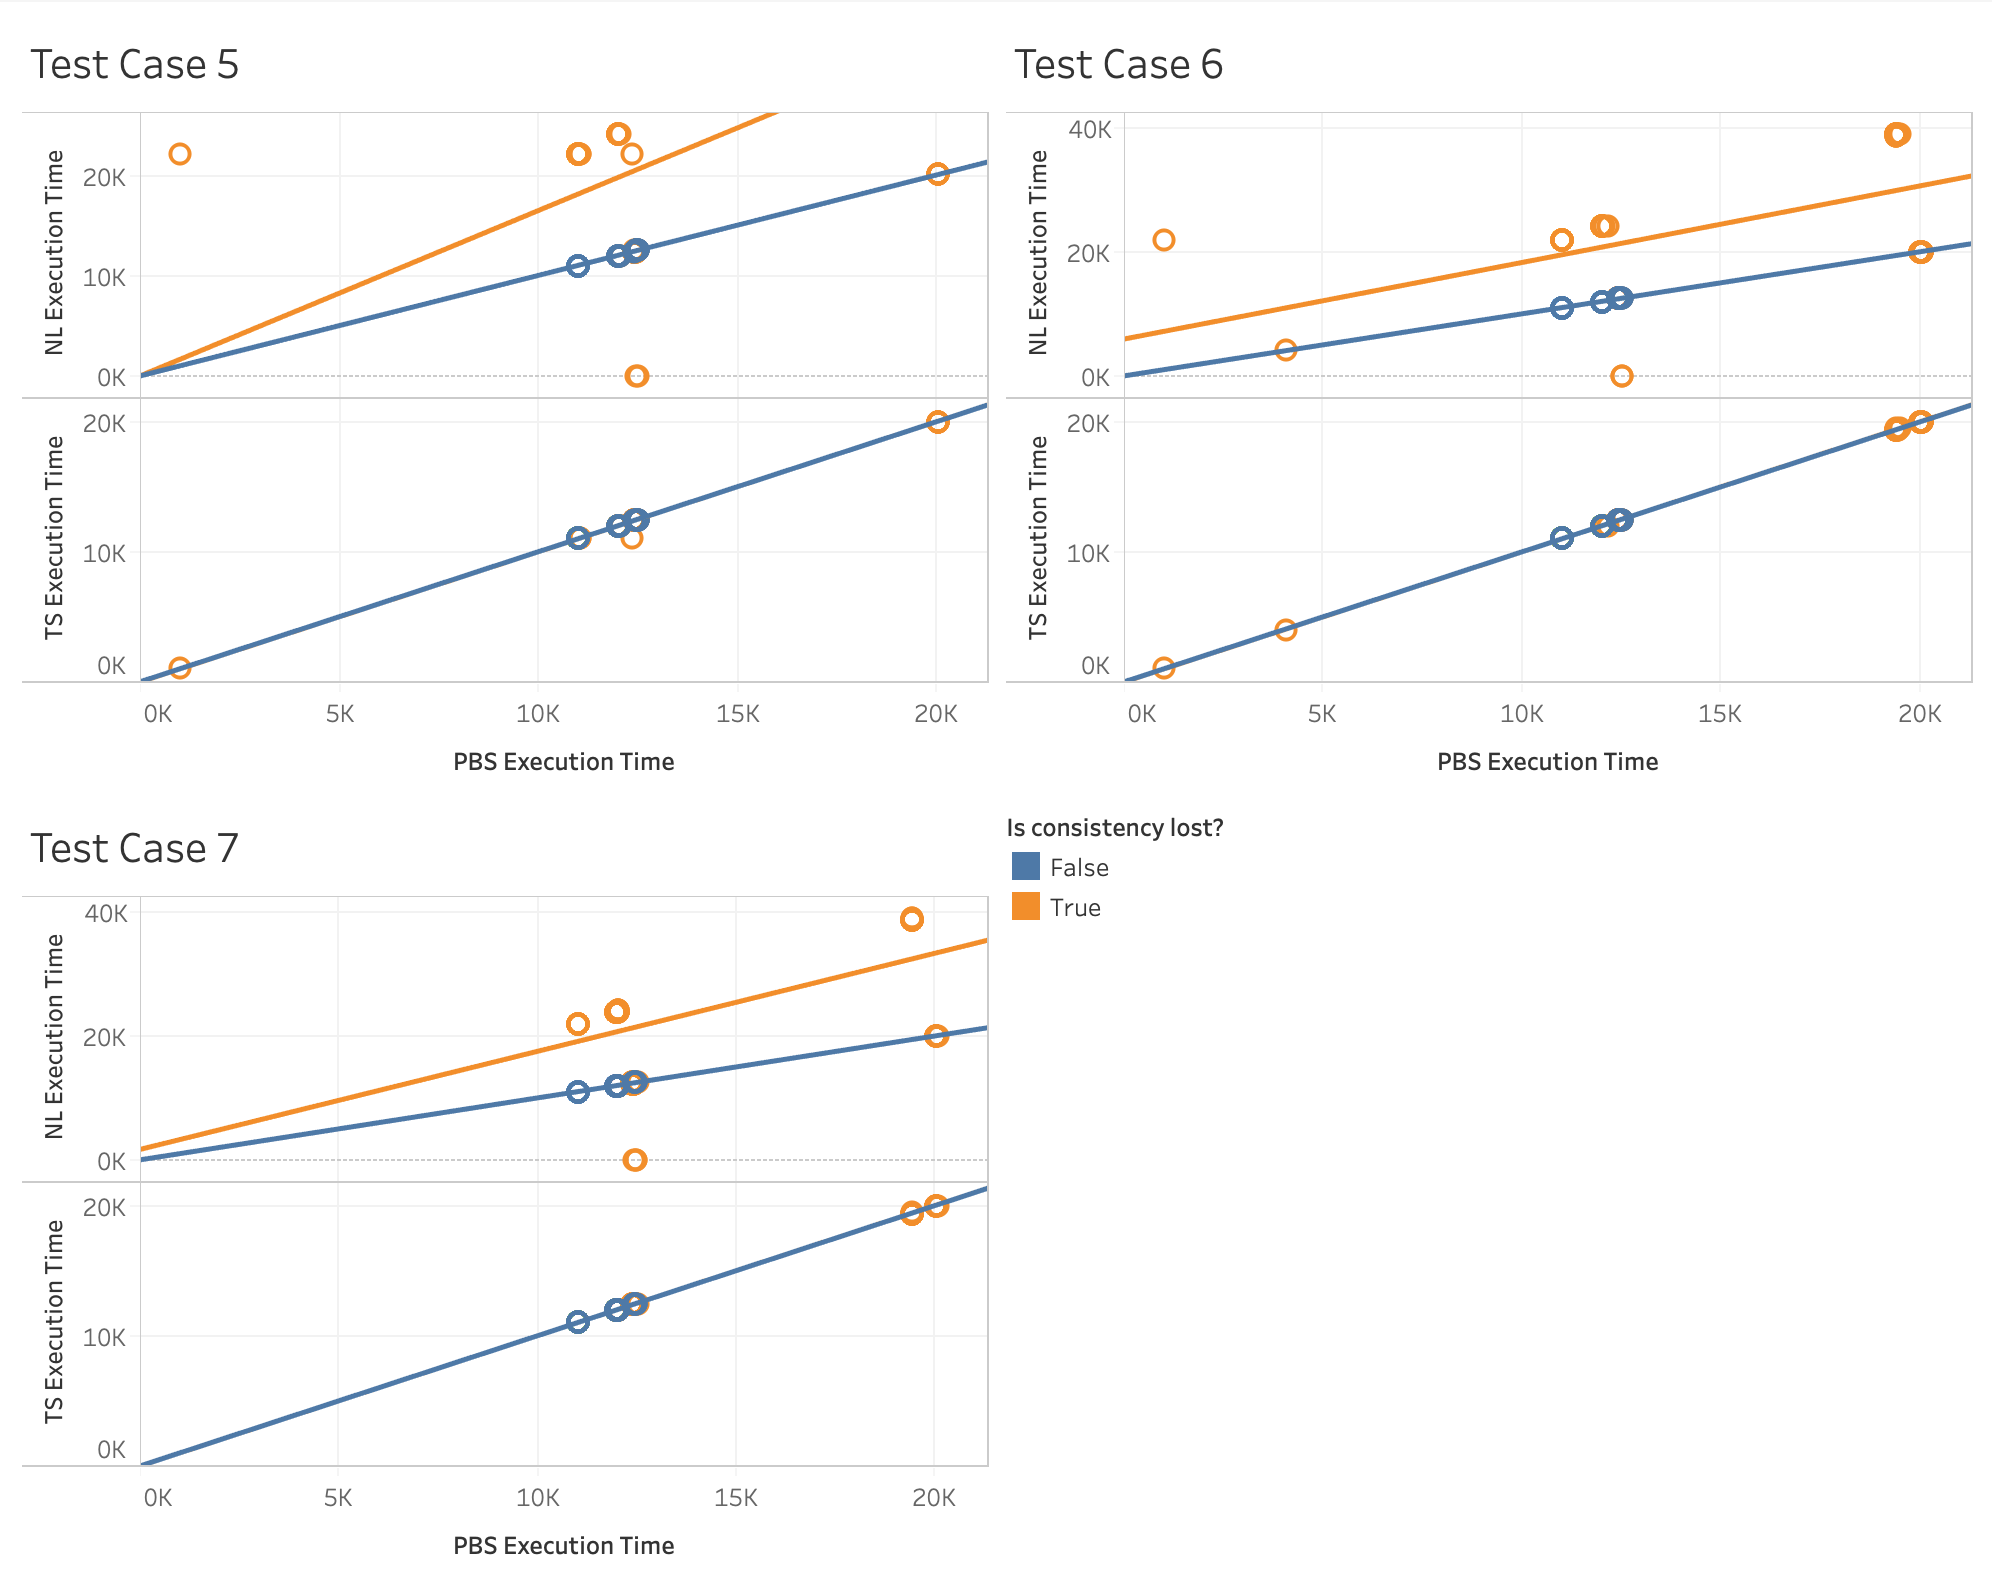
\includegraphics[scale=0.40]{images/Dashboard2_TL.png}
\caption{Consistency Lost/Kept for Test Cases 5-7}
\label{results:consistency_test_case_graphs_5_7}
\end{figure}

\section{Conclusion}
\label{pbs:conclusion}
In summary, transactions within a web service context have always been given a higher priority to efficiency over consistency, and for good reason. When web services are collaborated together by business process languages, the time it takes to complete can be a duration of hours and performance cannot be sacrificed. However, allowing the underlying database to reach an inconsistent state frequently is not acceptable. With the prediction-based solution, we ensure consistency without the performance hit of traditional locking. The three scheduler actions (\textit{grant, decline,} and \textit{elevate}) combined with the four transactional categories ($HCHE$, $HCLE$, $LCHE$, and $LCLE$) develop a solution that can easily be extended to a distributed web service context, in order to improve the current concurrency control mechanisms available today. Our ongoing work aims to prevent malicious transactions from corrupting databases in a web service environment. Liu and Jajodia proposed a multi-phase confinement system that provided a certain level of intrusion tolerance for database systems \cite{Liu_Intrusion}. We believe their model can be expanded using the metrics similar to the ones presented here.

\subsection{Concluding Remarks}
Now that we have established a foundation for prediction-based schedulers, we can now focus on the reputation of the transactions themselves. In the next chapter, this is where we will place our focus. Chapter \ref{chap:prediction_based_scheduler} presented the solution and operated under the assumption that the reputation of the transactions were already established. Chapter \ref{chap:dynamic_reputation} focuses on exactly how the transactions establish their reputation and also dynamically increase or decrease their reputation.

% Transactional correctness and consistency in web service based database transactions are still an after-thought. With the compensation transactions solution, having transactions generate inconsistent states has become acceptable. We show that the prediction-based performance metric that is proposed here is a scalable and efficient solution to web service transactions. This would drastically minimize the amount of compensation transactions needed to ensure consistency in concurrent database transactions. We also show that the solution will ensure a consistent state for transactions that have built a reputation for being reliable under the calculated performance metric.